\section{Bottomonia production mechanism in heavy ion collisions}
\label{sec:Bottomonia_hi}

\subsection{Theory overview}

\subsubsection{Sequential suppression and lattice QCD}
{\color{red} This subsection will include the details of the model by Strickland et. al. This
reference have most of the details about the model~\cite{Mocsy:2013syh}}
              
              
\subsubsection{Effect of nuclear PDFs on quarkonium production in nucleus-nucleus collisions}
{\color{red} This subsection will include the details of the models which use nuclear PDFs for quarkonia production
like EPS19 or Color Glass Condensate modes. etc.~\cite{}. These effects are small for the Upsilon sector. }


\subsubsection{Collisional dissociation of quarkonia from final-state interactions}

{\color{black}
                              
                             
  
                              
  \paragraph{Modification of quarkonia in the presence of QGP}
  In the kinetic approach \cite{Thews:2000rj}, the proper time $\tau$ evolution of the quarkonia 
  population $N_{Q}$
  is given by the rate equation 
  
  \begin{equation}\label{eqkin}
    {dN_{Q} \over d\tau}  =  - \lambda_D  \rho_g N_{Q} + \lambda_F {N_{q \bar{q}}^{2} \over V(\tau)},
  \end{equation}
  where $V(\tau)$ is the volume of the deconfined spatial region and $N_{q \bar{q}}$ is the number of initial 
  heavy quark pairs produced per event depending on the centrality defined by the number of participants
  $N_{\rm part}$.
  The $\lambda_{D}$ is the dissociation rate obtained by the dissociation cross section averaged over 
  the momentum 
  distribution of gluons and $\lambda_{F}$ is the formation rate obtained by the formation cross section 
  averaged over the momentum distribution of heavy quark pair $q$ and $\bar{q}$. 
  $\rho_g$ is the density of thermal gluons.
  The number of quarkonia at freeze-out time $\tau_f$ is given by the solution of Eq.~(\ref{eqkin}),
  \begin{equation}
    N_{Q}(p_T) = S(p_T) \,N_{Q}^{\rm PbPb}(p_T)+N_{Q}^F(p_T).
    \label{eqbeta}
  \end{equation}
  Here $N_{Q}^{\rm PbPb}(p_T)$ is the number of initially-produced quarkonia (including shadowing)
  as a function of $p_T$ and $S(p_T)$ is their survival probability from gluon collisions at freeze-out, 
  \begin{equation}
    S(p_T) = \exp \left( {-\int_{\tau_0}^{\tau_f}f(\tau) \lambda_{\rm D}(T,p_T)\,\rho_g(T)\,d\tau} \right).
  \end{equation}
  The temperature $T(\tau)$ and the QGP fraction $f(\tau)$ evolve from initial time $\tau_0$ 
  to freeze-out time $\tau_f$ due to expansion of the QGP. The initial temperature and the 
  evolution is dependent on collision centrality $N_{\rm part}$.
  $N_{Q}^F(p_T)$ is the number of regenerated quarkonia per event,
  \begin{equation}
    N_{Q}^F(p_T)=S(p_T)N_{q \bar{q}}^{2} \int_{\tau_0}^{\tau_f}{{\lambda_{\mathrm{F}}(T,p_T) \over V(\tau)\,S(\tau,p_T)} d\tau}.
  \end{equation}
  The nuclear modification factor ($R_{AA}$) can be written as 
  \begin{equation}
    R_{AA}(p_T)=S(p_T) \, R(p_T) + \frac{N_{Q}^F(p_T)}{N_{Q}^{pp}(p_T)}.
    \label{raa}
  \end{equation}
  Here $R(p_T)$ is the shadowing factor.
  $R_{AA}$ as a function of collision centrality, including regeneration, is
  \begin{equation}
    R_{AA}(N_{\rm part}) = \frac{\int_{p_{T\,\rm cut}} N_{Q}^{pp}(p_T)S(p_T)\, R(p_T) dp_T}{\int_{p_{T\,\rm cut}} N_{Q}^{pp}(p_T) dp_T} + 
    \frac{\int_{p_{T\, \rm cut}} N_{Q}^F(p_T) dp_T}{\int_{p_{T\, \rm cut}} N_{Q}^{pp}(p_T) dp_T}
    \label{raa2}
  \end{equation}
  Here $p_{T~{\rm cut}}$ defines the $p_T$ range for a given experimental acceptance.
  $N_{Q}^{pp}(p_T)$ is the unmodified $p_T$ distribution of quarkonia obtained by NLO 
  calculations and scaled to a particular centrality of the Pb+Pb collisions.
  
  The evolution of the system for each centrality bin is governed by
  an isentropic cylindrical expansion with volume element
  \begin{equation}
    V(\tau) = \tau\,\pi\,(R + {1\over 2} a_{T} \, \tau^2 )^{2},
  \end{equation}
  where $a_{T} = 0.1\,c^2$ fm$^{-1}$ is the transverse acceleration \cite{Zhao:2011cv}.
  The initial transverse size, $R$, as a function of centrality is
  \begin{equation}
    R(N_{\rm part}) = R_{0-5\%} \, \sqrt{N_{\rm part} \over (N_{\rm part})_{0-5\%} },
    \label{RVsNPart}
  \end{equation}
  where $R_{0-5\%} = 0.96\,R_{\rm Pb}$ and $R_{\rm Pb}$ is the radius of the lead nucleus.
  The evolution of entropy density for each centrality is obtained by entropy conservation, 
  $s(T)\,V(\tau)= s(T_0)\,V(\tau_0)$.
  The equation of state (EOS) obtained from Lattice QCD, along with a hadronic resonance gas, \cite{Huovinen:2009yb} 
  is used to obtain the temperature as a function of proper time $\tau$.
  The initial entropy density for each centrality is calculated using 
  \begin{equation}
    s(\tau_0) = s(\tau_0)|_{0-5\%} \left(\frac{dN/d\eta}{N_{\rm part}/2}\right)\left(\frac{dN/d\eta}{N_{\rm part}/2}\right)^{-1}_{0-5\%}.
    \label{TempNpart}
  \end{equation}
  Measured values of $(dN/d\eta)/(N_{\rm part}/2)$ as a function of $N_{\rm part}$ 
  {\color{black} \cite{Aamodt:2010cz,Chatrchyan:2011pb}} are used in the calculations.
  The initial entropy density, $s(\tau_0)|_{0-5\%}$, for 0-5\% centrality is 
  \begin{eqnarray}
    s(\tau_0)|_{0-5\%}  = {a_{m} \over V(\tau_0)|_{0-5\%}}   \left(\frac{dN}{d\eta}\right)_{0-5\%} . 
    \label{TempVsMult}
  \end{eqnarray}  
  Here $a_m$ {\color{black}(= 5)} is a constant which relates the total entropy to the total 
  multiplicity $dN/d\eta$. It is obtained from hydrodynamic calculations \cite{Shuryak:1992wc}.
  {\color{black}
    We estimate the initial temperature, $T_0$, in the 0-5$\%$ most central collisions
    from the total multiplictity in the rapidity region of interest, assuming that the initial time is
    $\tau_0 = 0.3$ fm/$c$ over all rapidity.  The total multiplicity in a given rapidity region is
    3/2 times the charged particle multiplicity in Pb+Pb collisions at 2.76 TeV.  With the lattice
    EOS, at midrapidity, with $(dN_{\rm ch}/d\eta)_{0-5\%} = 1600$~\cite{Aamodt:2010cz,Chatrchyan:2011pb}, 
    we find $T_0 = 0.484$ GeV.  Likewise, at forward rapiidity, $2.5 \leq y \leq 4$~\cite{Abbas:2013bpa}, 
    $T_0 = 0.427$ GeV.}
  The (proper) time evolution of temperature is shown in Fig.~\ref{fig:TauVsTemp}(a) 
  and that of QGP fraction in Fig.~\ref{fig:TauVsTemp}(b), in the case of the most central (0-5$\%$) collisions.
  Here we compare the evolution obtained with longitudinal and cylindrical expansions using 
  both a first order and the lattice EOS. 
  For the first order EOS, $T_c$ = 0.170 GeV. The QGP fraction goes from 1 to 0 at $T_c$ 
  assuming a mixed phase of QGP and hadrons. The QGP fraction in case of lattice EOS governs the 
  number of degrees of freedom, decided by the entropy density. It is fixed to unity above an entropy density 
  corresponding to a 2-flavour QGP and fixed to zero below entropy density for a hot 
  resonance gas. The freeze out temperature in all cases is $T_f=0.140$ GeV.  
  
  \begin{figure}
    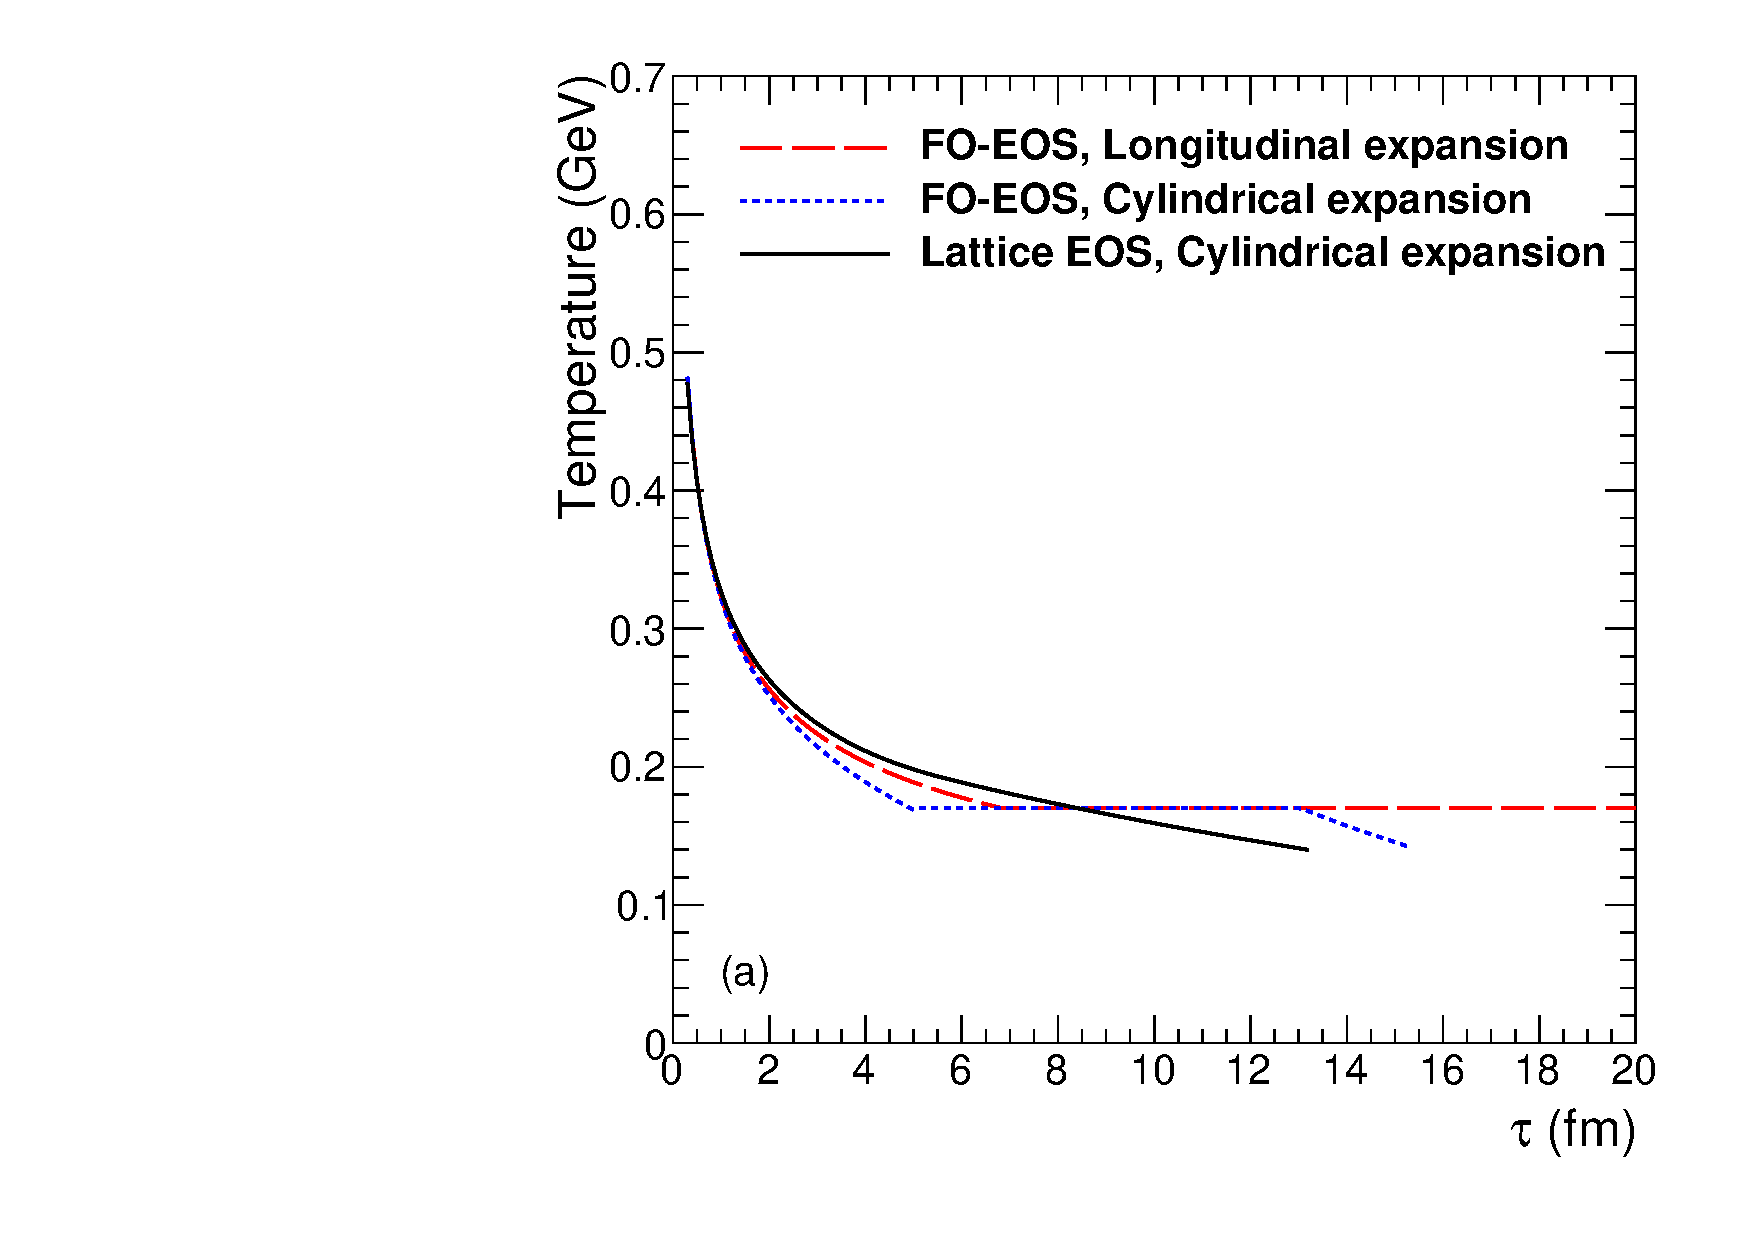
\includegraphics[width=0.49\textwidth]{Figures/Quarkonia_276TeV/Fig1a_TauVsTemp.pdf}
    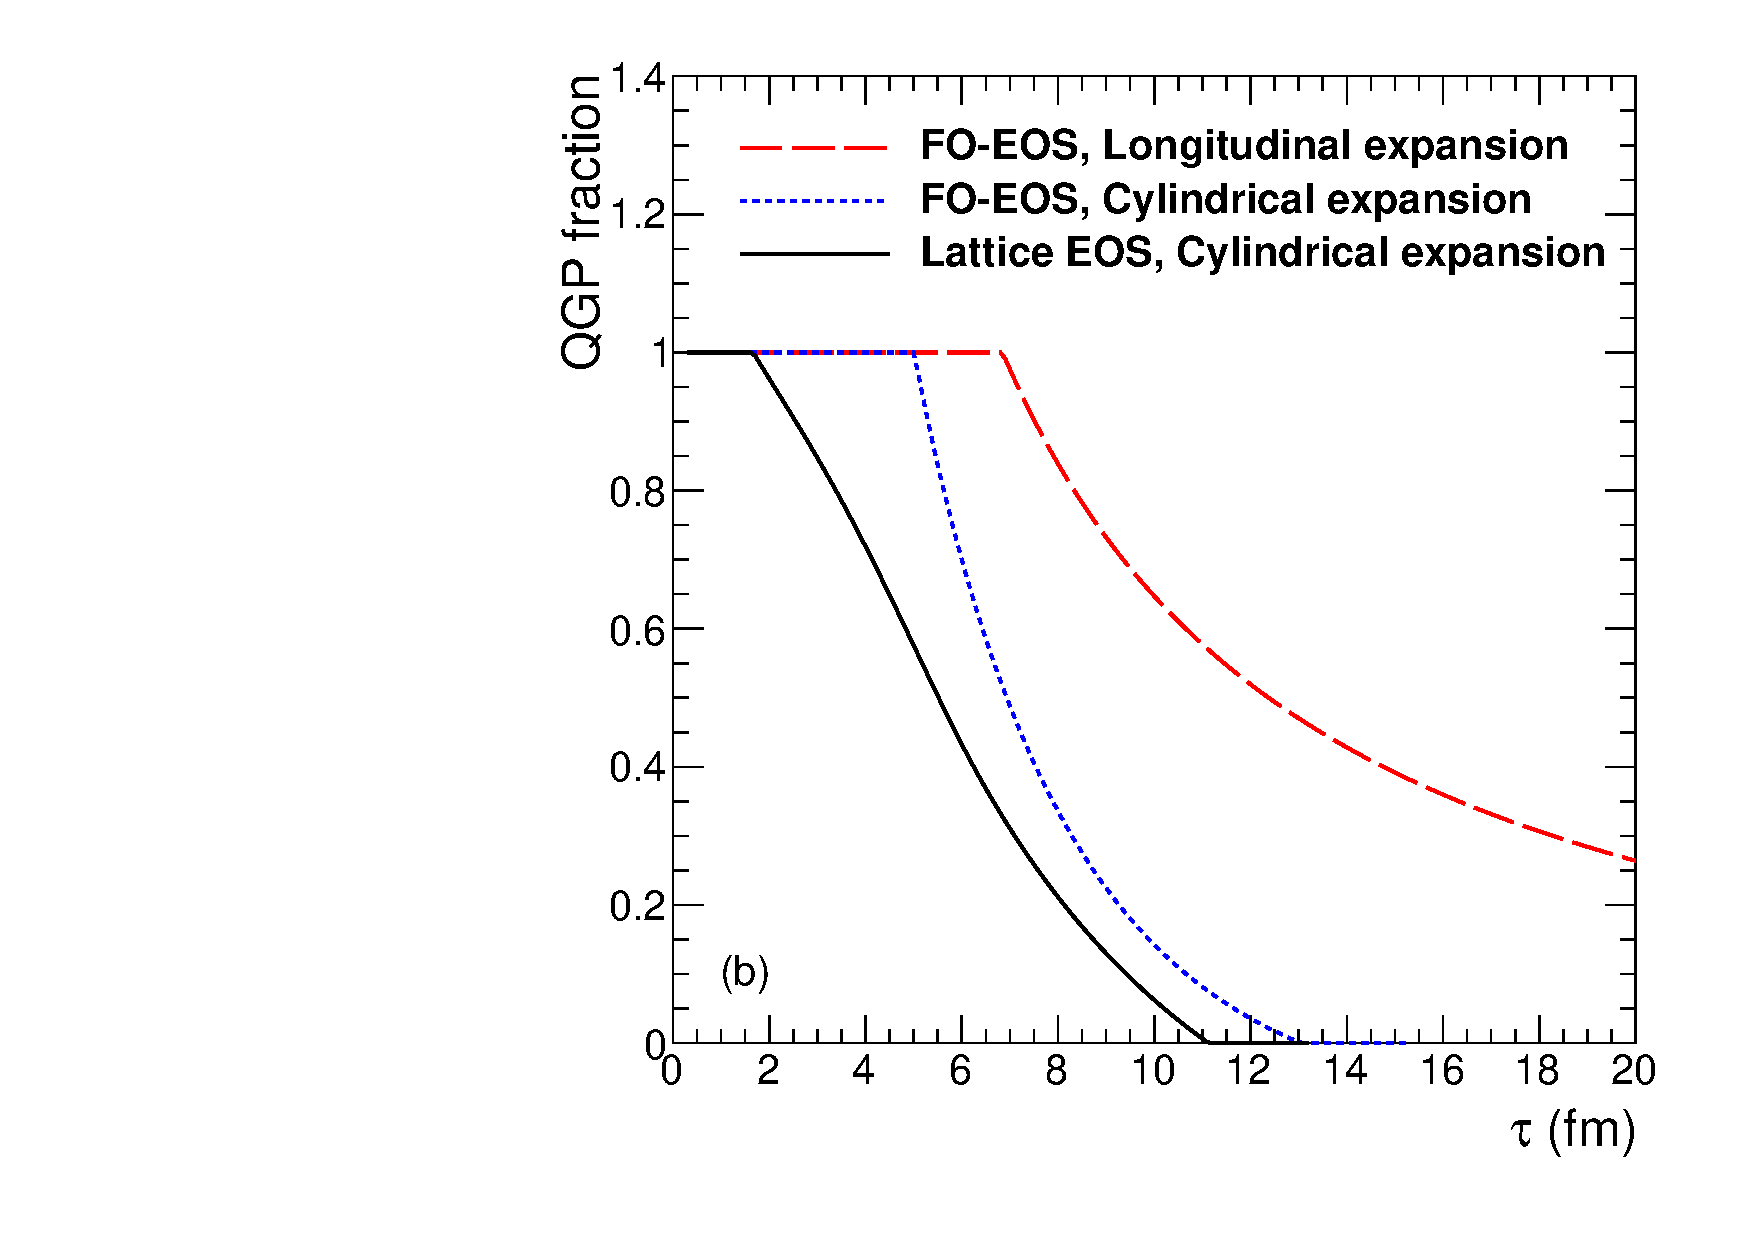
\includegraphics[width=0.49\textwidth]{Figures/Quarkonia_276TeV/Fig1b_TauVsFQGP.pdf}
    \caption{(Color online) (a) Temperature and (b) QGP fraction in the system as a function of proper 
      time $\tau$ in case of the most central (0-5$\%$) collisions for longitudinal and cylindrical expansions 
      using first order and lattice equation of state.}
    \label{fig:TauVsTemp}
  \end{figure}
  %%%%%%%%%%%%%%%%%%%%%%%%%%%%%%%%%%%%%%%%%%%%%%%%%%%%%%%%%%%%%%%%%%%%%%%%%%%%%%%%%%%%%%%%%%%%%%%%%
  \subsection{Dissociation Rate}
  In the color dipole approximation, the gluon dissociation cross section as function of gluon energy, $q^0$,
  in the quarkonium rest frame is~\cite{Bhanot:1979vb}
  \begin{equation}
    \sigma_{D}(q^{0}) = {8\pi \over 3} \, {16^2 \over 3^2} {a_0 \over m_q}  \frac{(q^0/\epsilon_0 - 1)^{3/2}} {(q^0/\epsilon_0)^5},
  \end{equation}
  where $\epsilon_0$ is the quarkonia binding energy and $m_q$ is the charm/bottom quark mass 
  and $a_0=1/\sqrt{m_q\epsilon_0}$.
  The values of $\epsilon_0$ are taken as 0.64 and 1.10 GeV for the ground states, $\Jpsi$ and $\Upsilon$(1S),
  respectively \cite{Karsch:1987pv}.
  For the first excited state of bottomonia, $\Upsilon$(2S), we use dissociation
  cross section from Ref.~\cite{Arleo:2001mp}.
  
  Figure \ref{fig:SigmaDQ0} shows the gluon dissociation cross sections of $\Jpsi$ and $\Upsilon$(1S)
  as a function of gluon energy. The dissociation cross section is zero when the gluon energy is less 
  than the binding energy of the quarkonia. It increases with gluon energy and reaches a maximum at 1.2 (1.5) GeV for 
  $\Jpsi~(\Upsilon(1{\rm S}))$. At higher gluon energies, the interaction probability decreases. The gluon energy $q^0$ 
  is related to the square of the center of mass energy $s$, of the quarkonium-gluon system by
  \begin{eqnarray}
    q^{0} = \frac{s-M_{Q}^{2}}{2\,M_{Q}}
  \end{eqnarray}  
  where $s=M_{Q}^{2} + 2  p_g \, \sqrt{M_{Q}^2 + p^2} - 2  p_g \, p \, {\rm cos\theta}$, and $M_{Q}$ and $p$ 
  are mass and momentum of quarkonium and $\theta$ is angle between the quarkonium and the gluon.
  We calculate the dissociation rate as a function of quarkonium momentum 
  by integrating the dissociation cross section over thermal gluon momentum 
  distribution $f_{g}(p_g)$,   
  \begin{eqnarray}
    \lambda_{D} \rho_{g}  & = & \langle \sigma v_{\rm rel} \rangle \,\rho_{g}  = \frac{g_g}{(2\pi)^{3}} \int d^{3}p_g \, f_{g}(p_g)  \, \sigma_{D}(s) v_{\rm rel}(s)  \nonumber \\ 
    & = & \frac{g_g}{(2\pi)^{3}} \int dp_g 2\pi p_g^{2} f_{g}(p_g) \int d\,{\rm cos\theta}\,\sigma_{D}(s)\,v_{\rm rel}(s),
  \end{eqnarray}
  where $\sigma_{D}(s) = \sigma_{D}(q^0(s))$.
  The relative velocity, $v_{\rm rel}$, between the quarkonium and the gluon is
  \begin{eqnarray}
    v_{\rm rel}  = {s- M_{Q}^{2} \over 2  p_g\sqrt{M_{Q}^2 + p^2}}.  
    \label{eq7}
  \end{eqnarray}
  The $\Jpsi$ gluon dissociation rates as a function of $T$ are shown in 
  Fig.~\ref{fig:DRateVsTempAndPt}(a) and as a function of $p_T$ in Fig.~\ref{fig:DRateVsTempAndPt}(b).
  The dissociation rate increases with temperature due to the increase in gluon density. 
  The dissociation rate is maximum when the quarkonium is at rest and decreases with $p_T$.

  
  \begin{figure}
    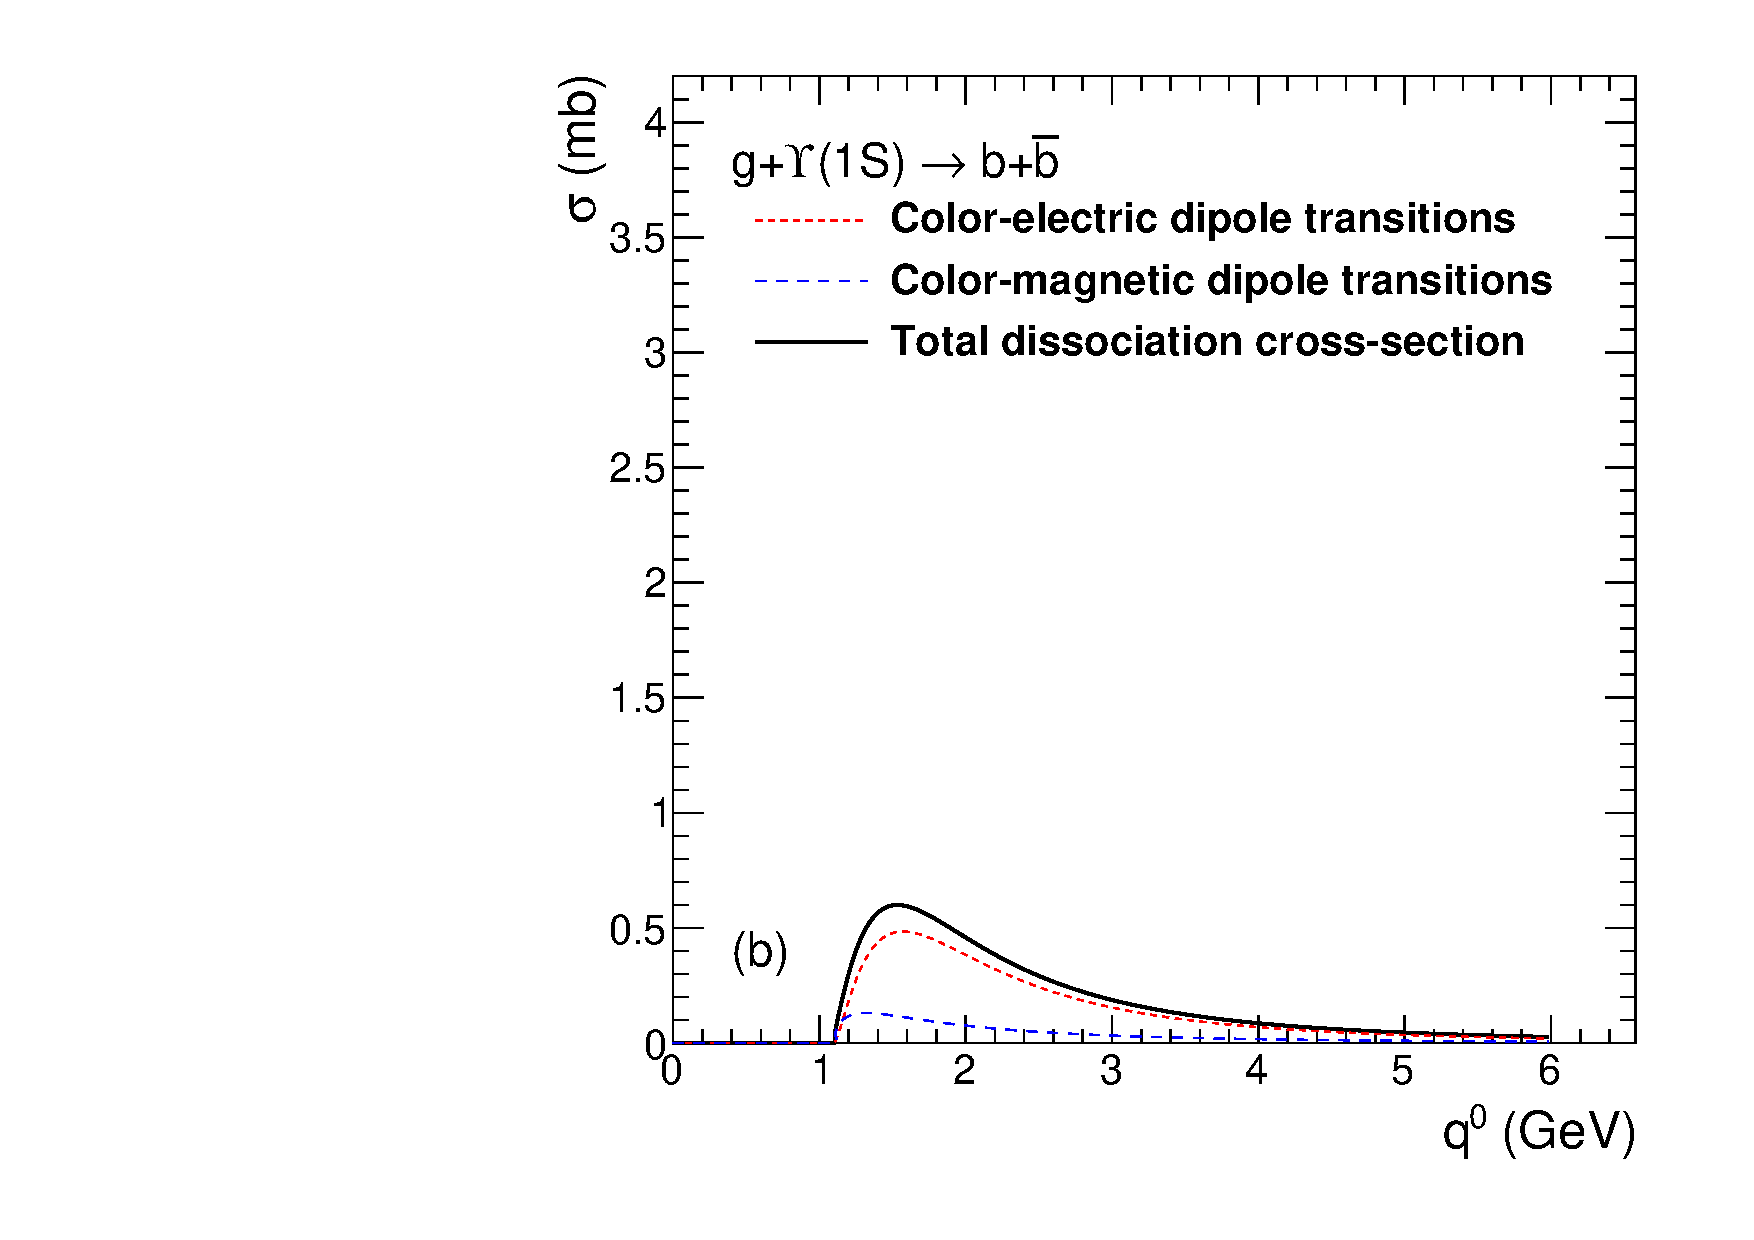
\includegraphics[width=0.60\textwidth]{Figures/Quarkonia_502TeV/Fig1b_Y1S_SigmaDq0.pdf}
    \caption{(Color online) Gluon dissociation cross section of quarkonia as a function of gluon energy ($q^{0}$) in
      quarkonia rest frame.}
    \label{fig:SigmaDQ0}
  \end{figure}
  


  \begin{figure}
    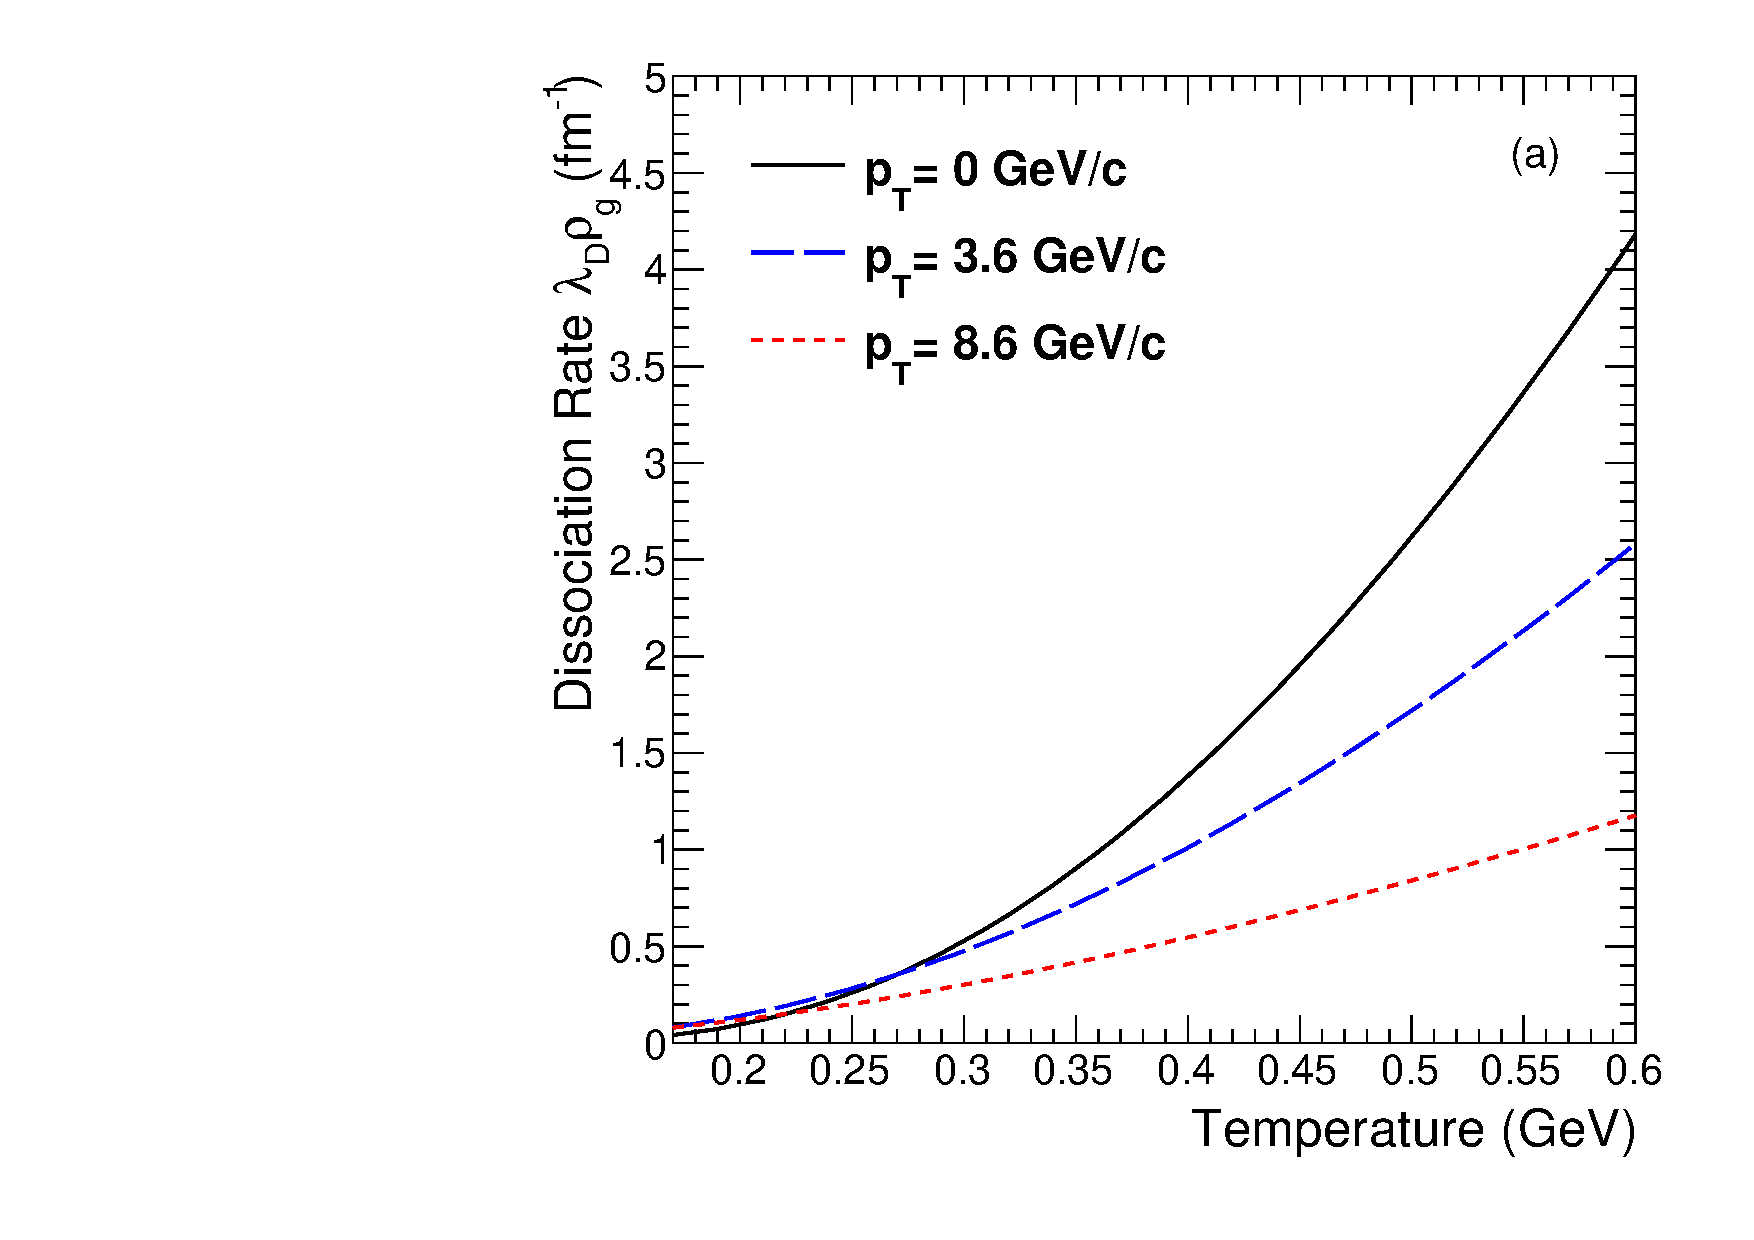
\includegraphics[width=0.49\textwidth]{Figures/Quarkonia_276TeV/Fig3a_DRateVsT.pdf}
    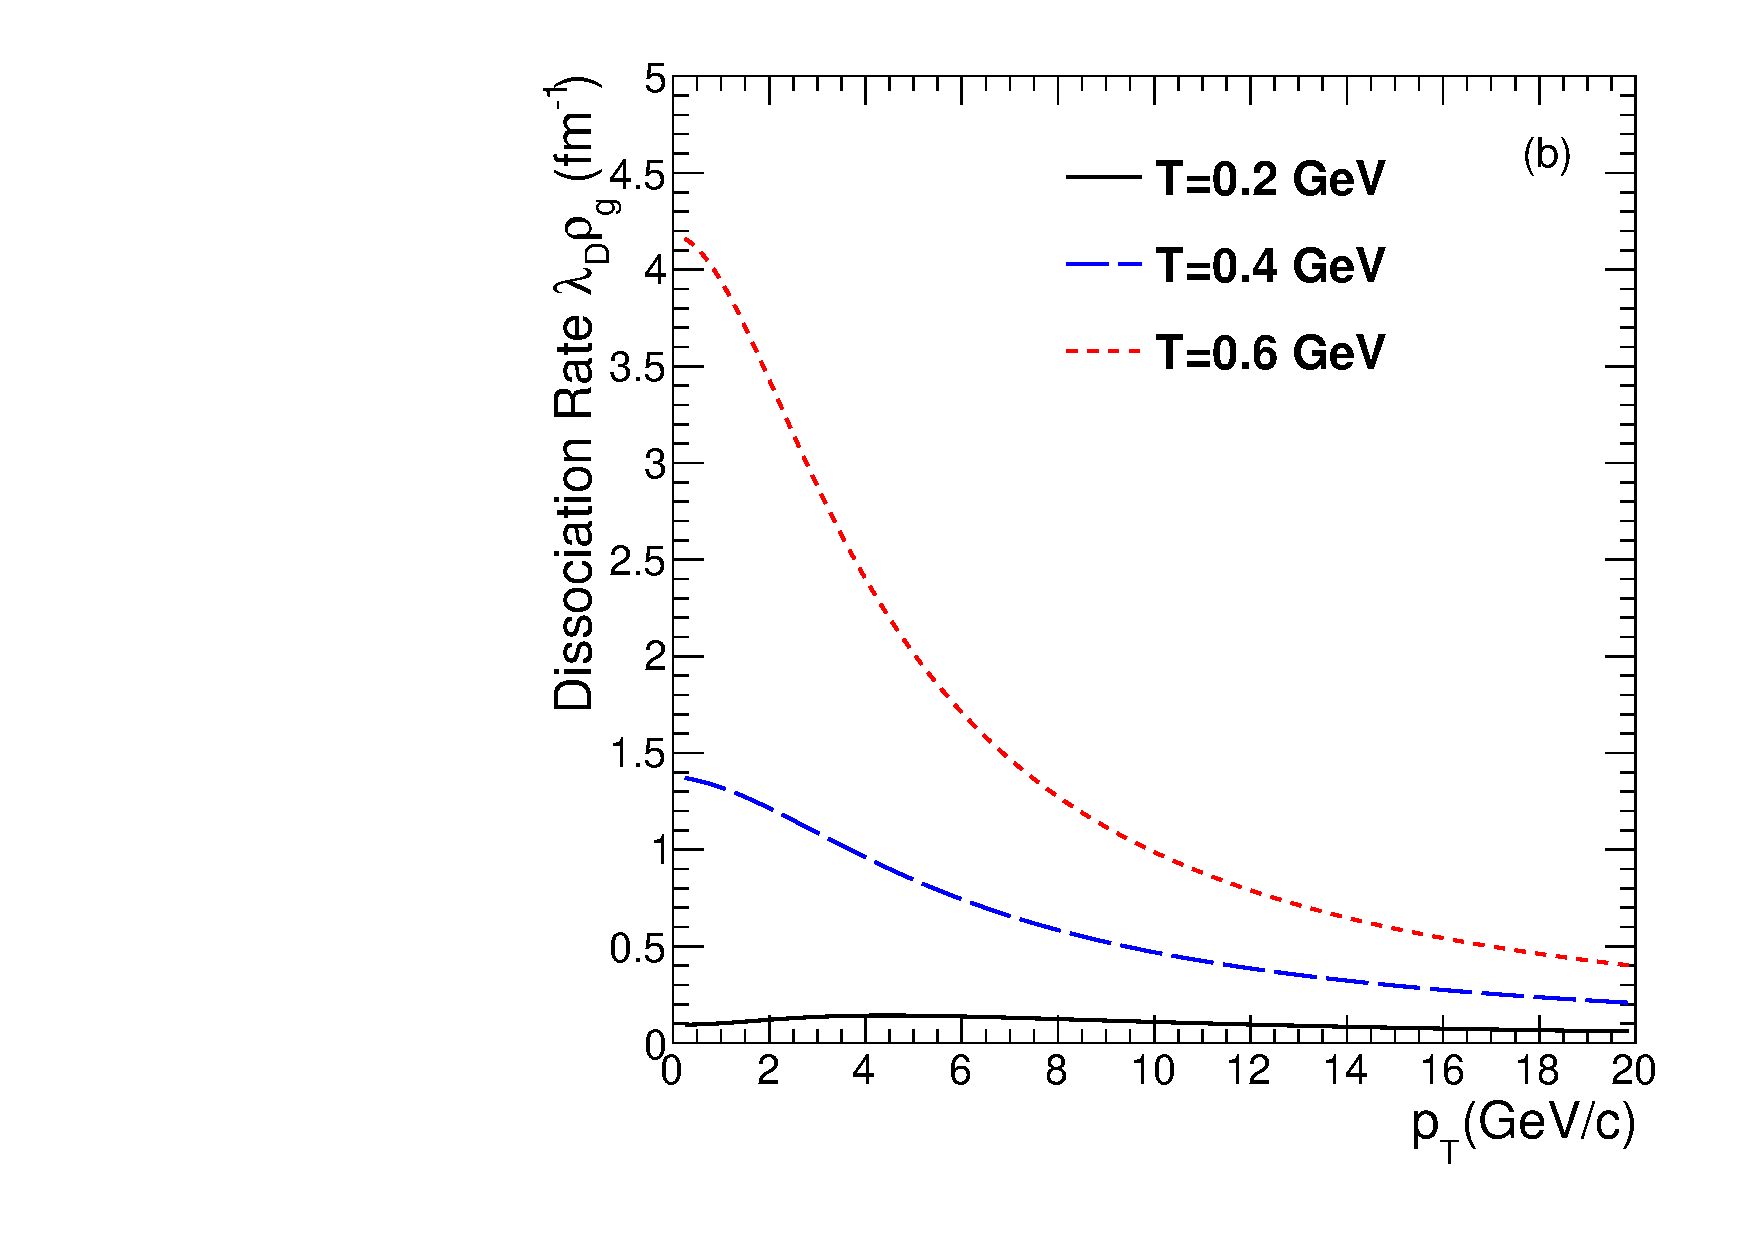
\includegraphics[width=0.49\textwidth]{Figures/Quarkonia_276TeV/Fig3b_DRateVsPt.pdf}
    \caption{(Color online) Gluon dissociation rate of $\Jpsi$ as a function of (a) temperature and  
      (b) transverse momentum.}
    \label{fig:DRateVsTempAndPt}
  \end{figure}
  \subsection{Formation Rate}
  We can calculate the formation cross section from the dissociation cross section using detailed balance~\cite{Thews:2000rj,Thews:2005vj},
  \begin{equation}
    \sigma_{F} = \frac{48}{36}\,\sigma_{D}(q^0)\frac{(s-M_{Q}^2)^{2}}{s(s-4m_q^{2})}.
  \end{equation}
  The formation rate of quarkonium with momentum {\bf p} can be written as
  \begin{equation}
    \frac{d\lambda_{F}}{d{\rm\bf p}} = \int \,d^{3}p_1 \,d^{3}p_2 \,\sigma_{F}(s)\, v_{\rm rel}(s)\,f_{q}(p_1)\, f_{\bar{q}} (p_2)\,\delta({\rm\bf p}-( {\rm\bf p_1} + {\rm\bf p_2} )).
  \end{equation}
  Here $f_{q/\bar{q}}(p)$ are taken as thermal distribution function of  $q/\bar{q}$ which are 
  normalized to one, $\int f_{q}(p) d^{3}p  = 1 $ and $v_{\rm rel}$ is relative velocity of the
  $q\bar{q}$ quark pair,
  \begin{eqnarray}
    v_{\rm rel} &=& {\sqrt{(p_{1}.p_{2})^{2} - m_q^{4} } \over E_{1} \, E_{2}}. %\nonumber \\
  \end{eqnarray}
  Here $p_1 = (E_1,{\bf p_{1}})$ and $p_{2} = (E_{2},{\bf p_{2}})$ are the four momenta of the heavy quark and 
  antiquark respectively.
  Figure \ref{fig:ForRateVsTempAndPt} (a) shows the variation of the formation rate as a function 
  of $T$ and Fig.~\ref{fig:ForRateVsTempAndPt} (b) shows as a function of $\Jpsi$ $p_T$.
  The $\Jpsi$ generated from recombination of uncorrelated heavy quark pairs will have 
  softer $p_{T}$ distributions than those of $\Jpsi$'s coming from the initial hard scatterings.
  Thus the effect of recombination will be important only at low $p_T$.
  
  \begin{figure}
    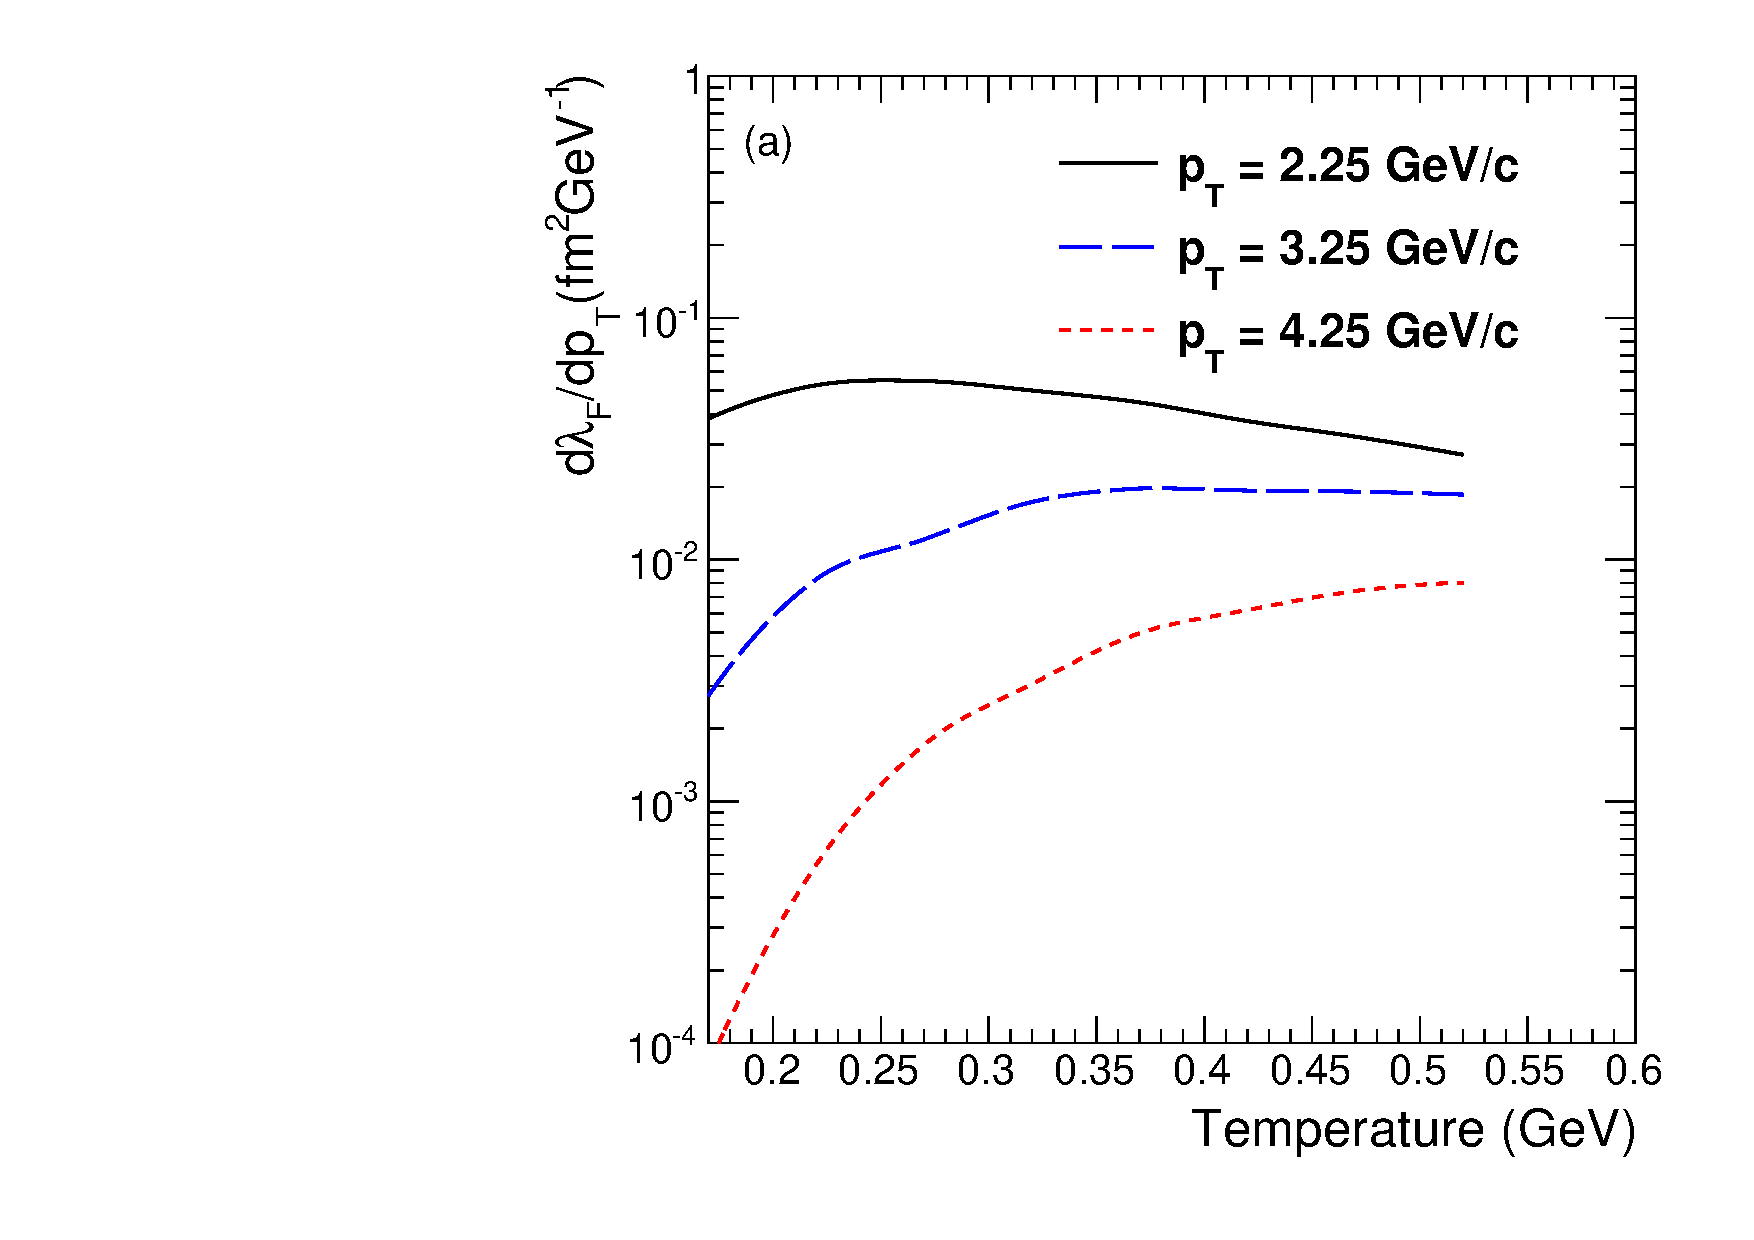
\includegraphics[width=0.49\textwidth]{Figures/Quarkonia_276TeV/Fig4a_FRateVsT.pdf}
    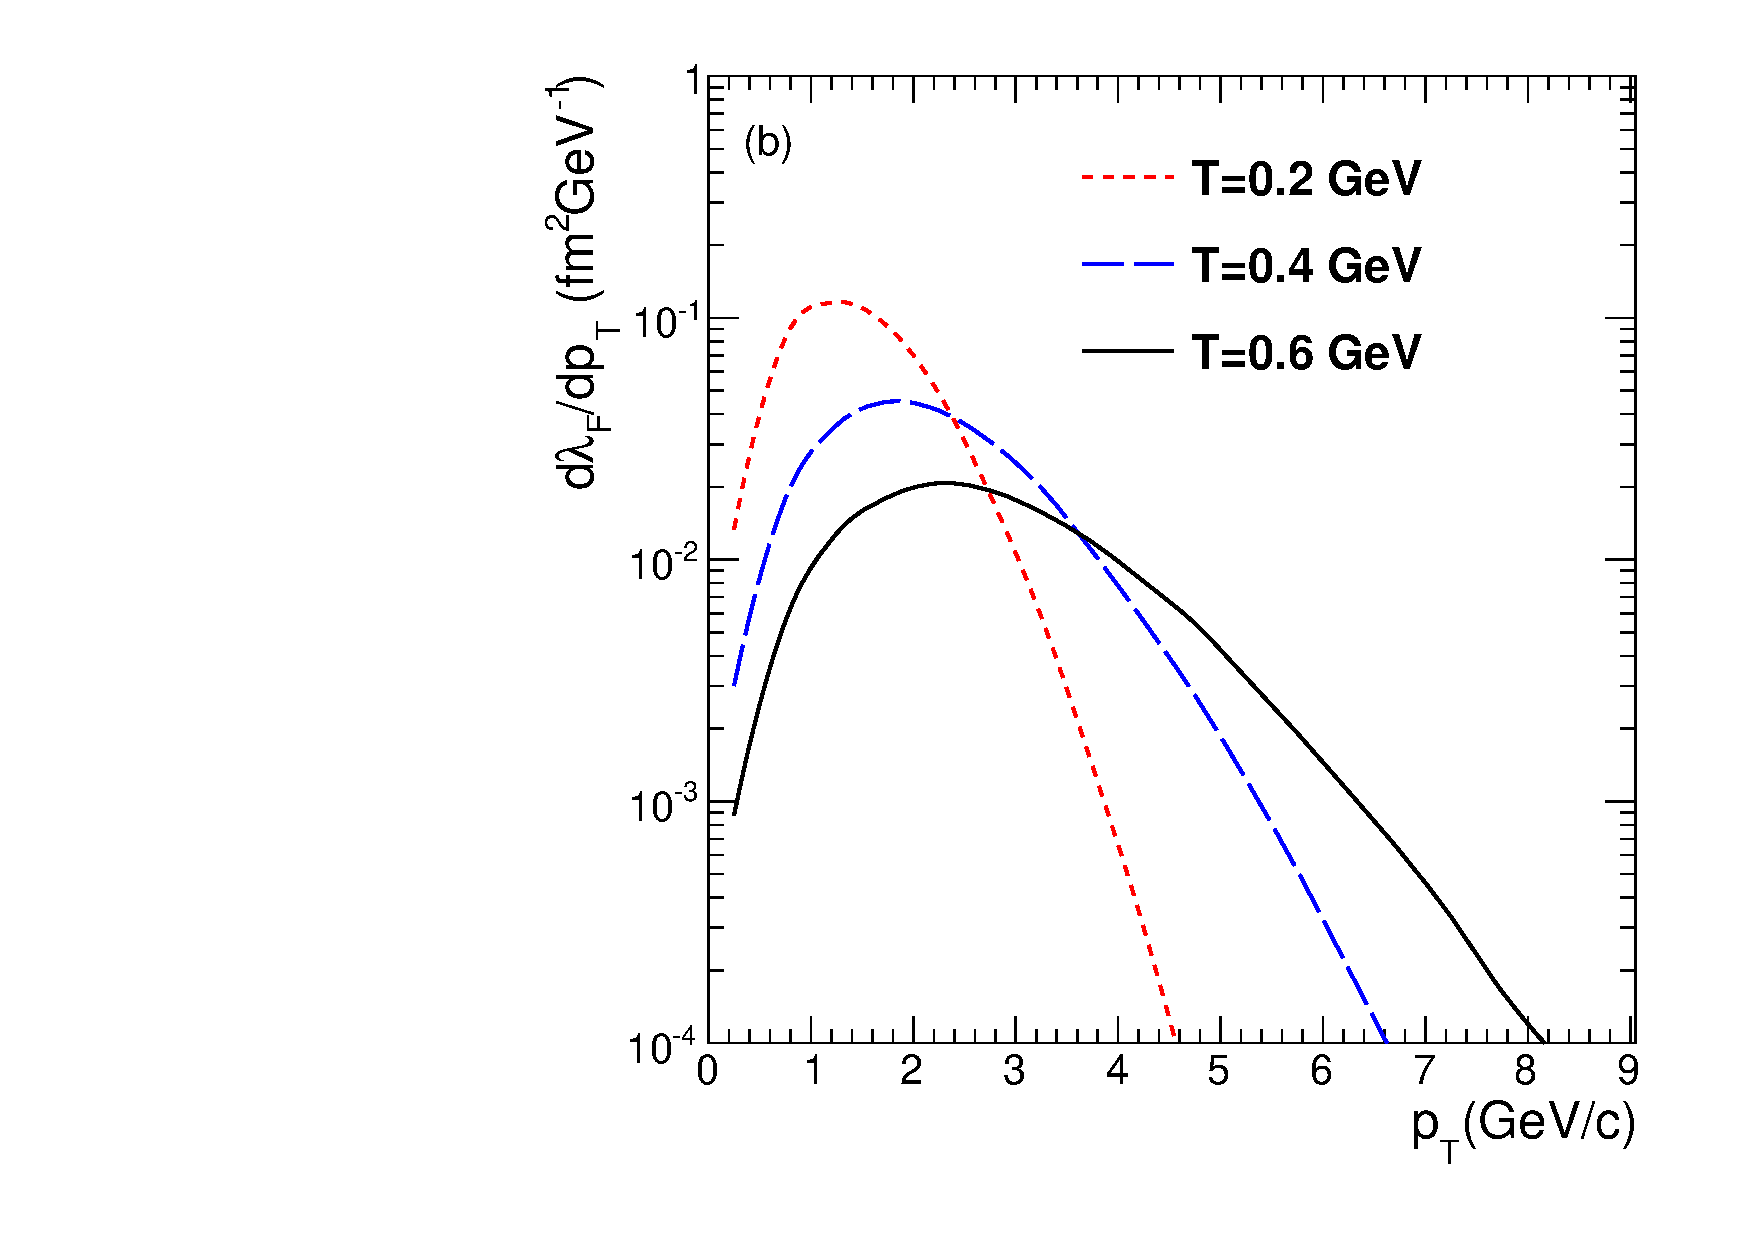
\includegraphics[width=0.49\textwidth]{Figures/Quarkonia_276TeV/Fig4b_FRateVsPt.pdf}
    \caption{(Color online) Formation rate of  $\Jpsi$ as a function of (a) temperature and 
      (b) transverse momentum.}
    \label{fig:ForRateVsTempAndPt}
  \end{figure}
  
  
  \begin{figure}
    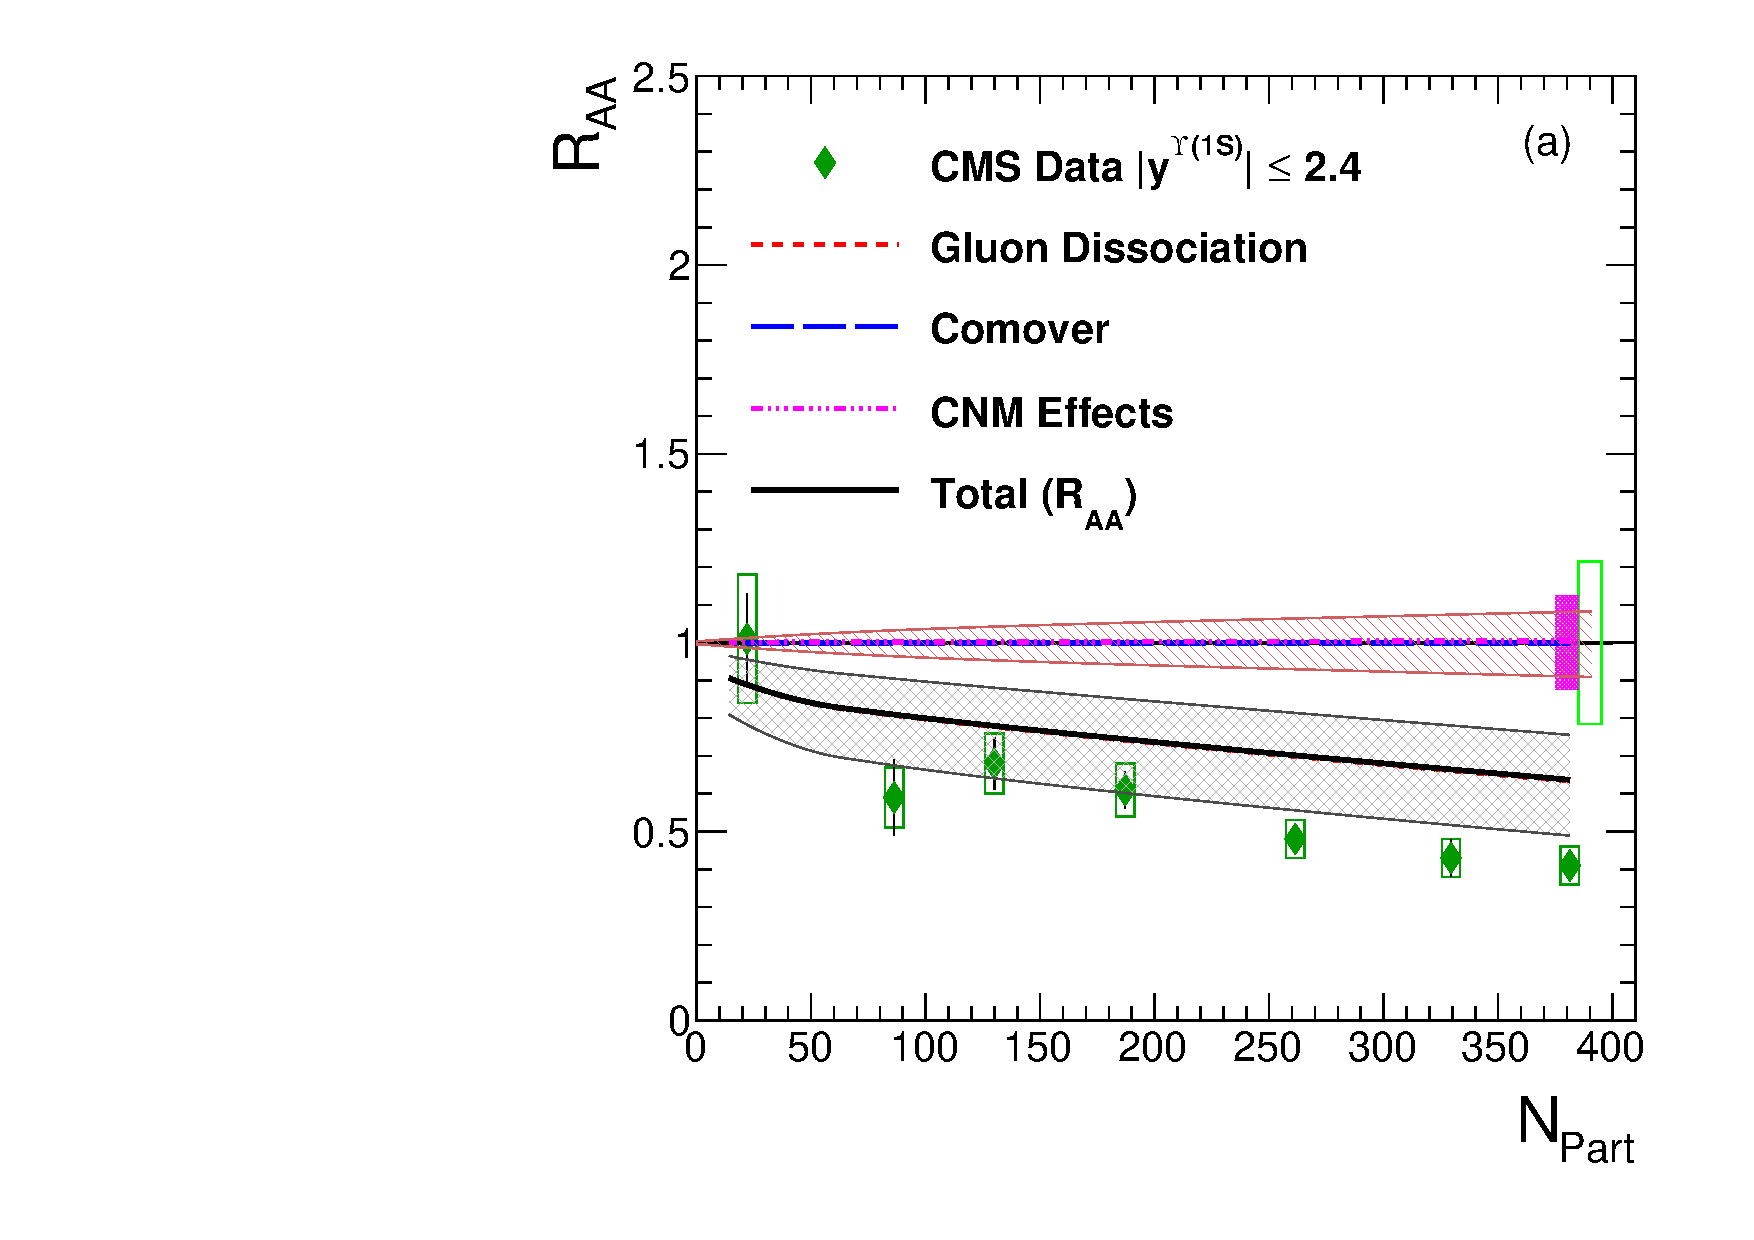
\includegraphics[width=0.49\textwidth]{Figures/Quarkonia_276TeV/Fig8a_CMS_Y1SRAANPart.pdf}
    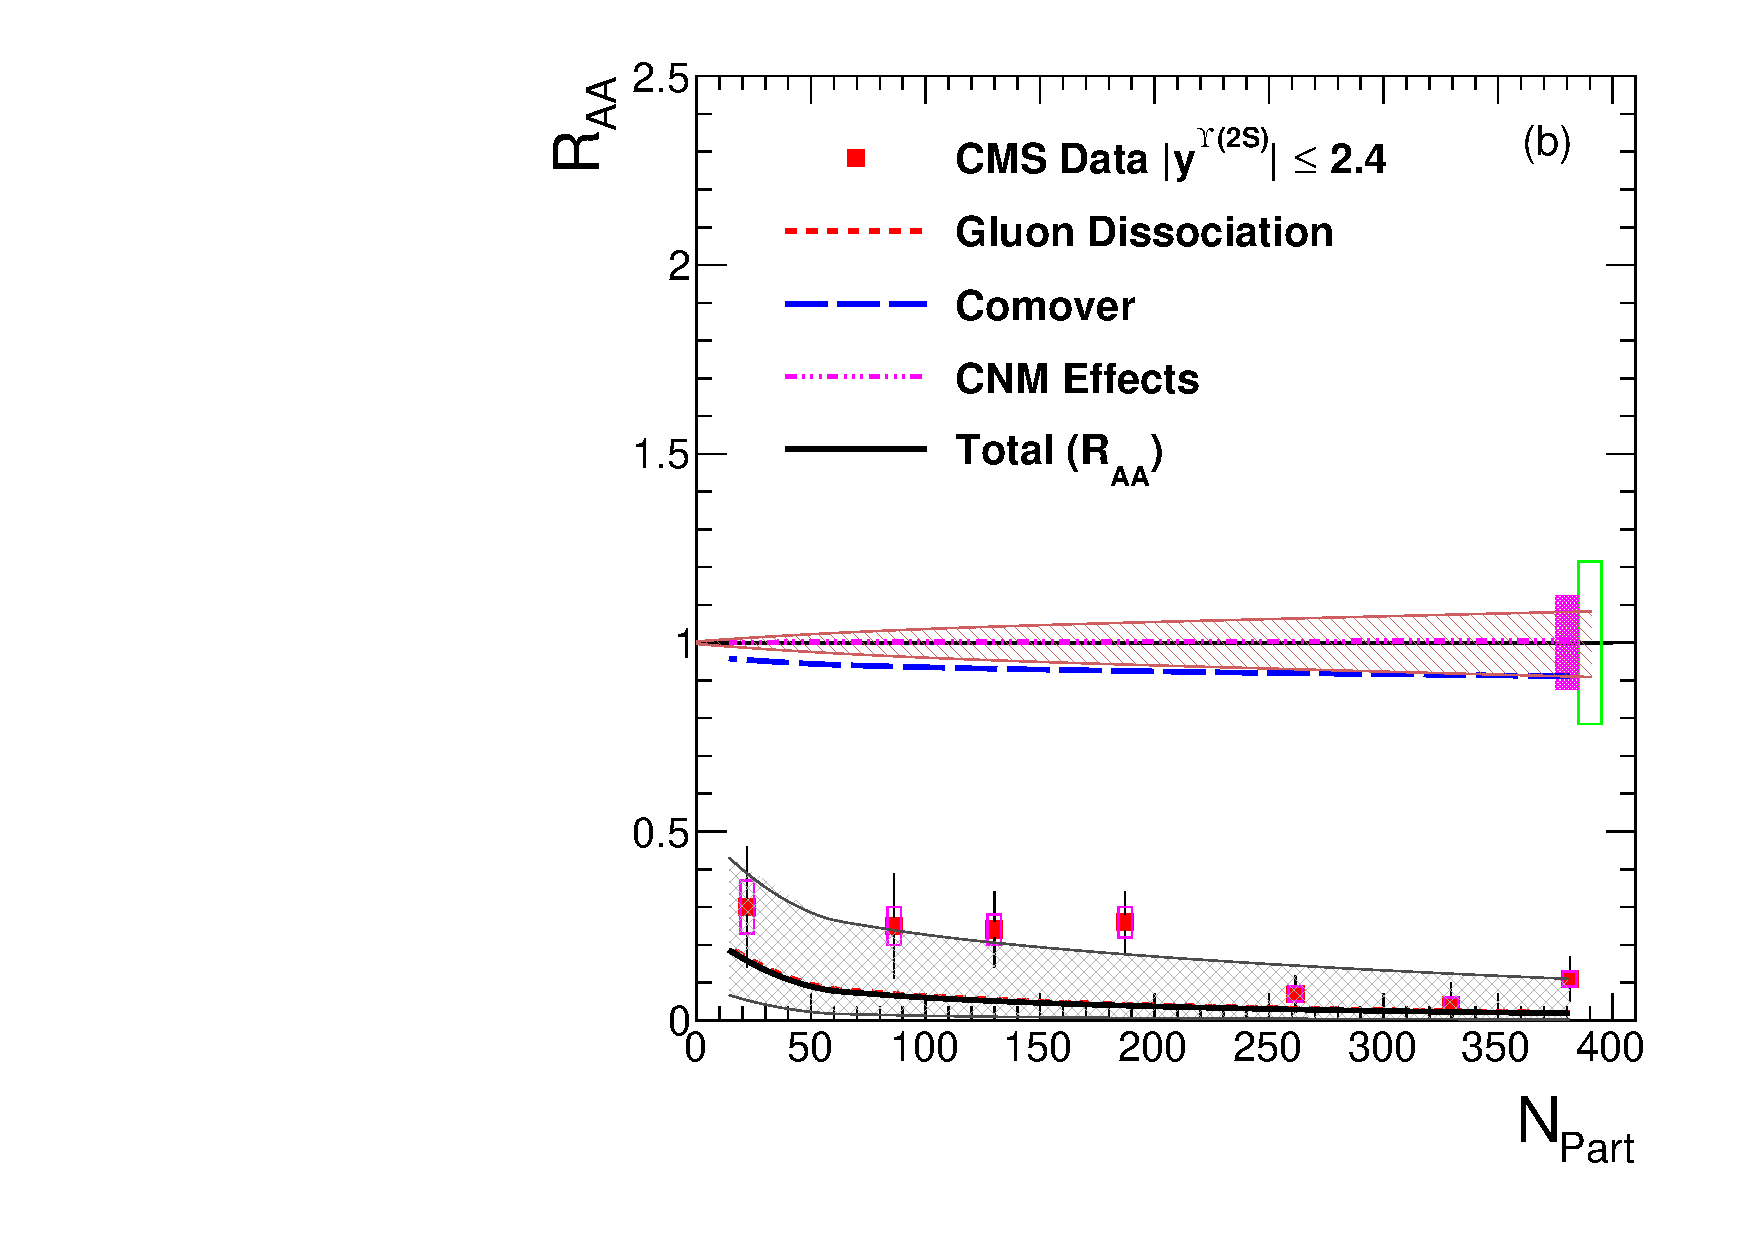
\includegraphics[width=0.49\textwidth]{Figures/Quarkonia_276TeV/Fig8b_CMS_Y2SRAANPart.pdf}
    \caption{(Color online) Calculated nuclear modification factor ($R_{AA}$) compared with CMS 
      (a) $\Upsilon$(1S) and (b) $\Upsilon$(2S) measurements. Regeneration is assumed to be negligible. }
    \label{fig:UpsilonRaa}
  \end{figure}
  \begin{figure}
    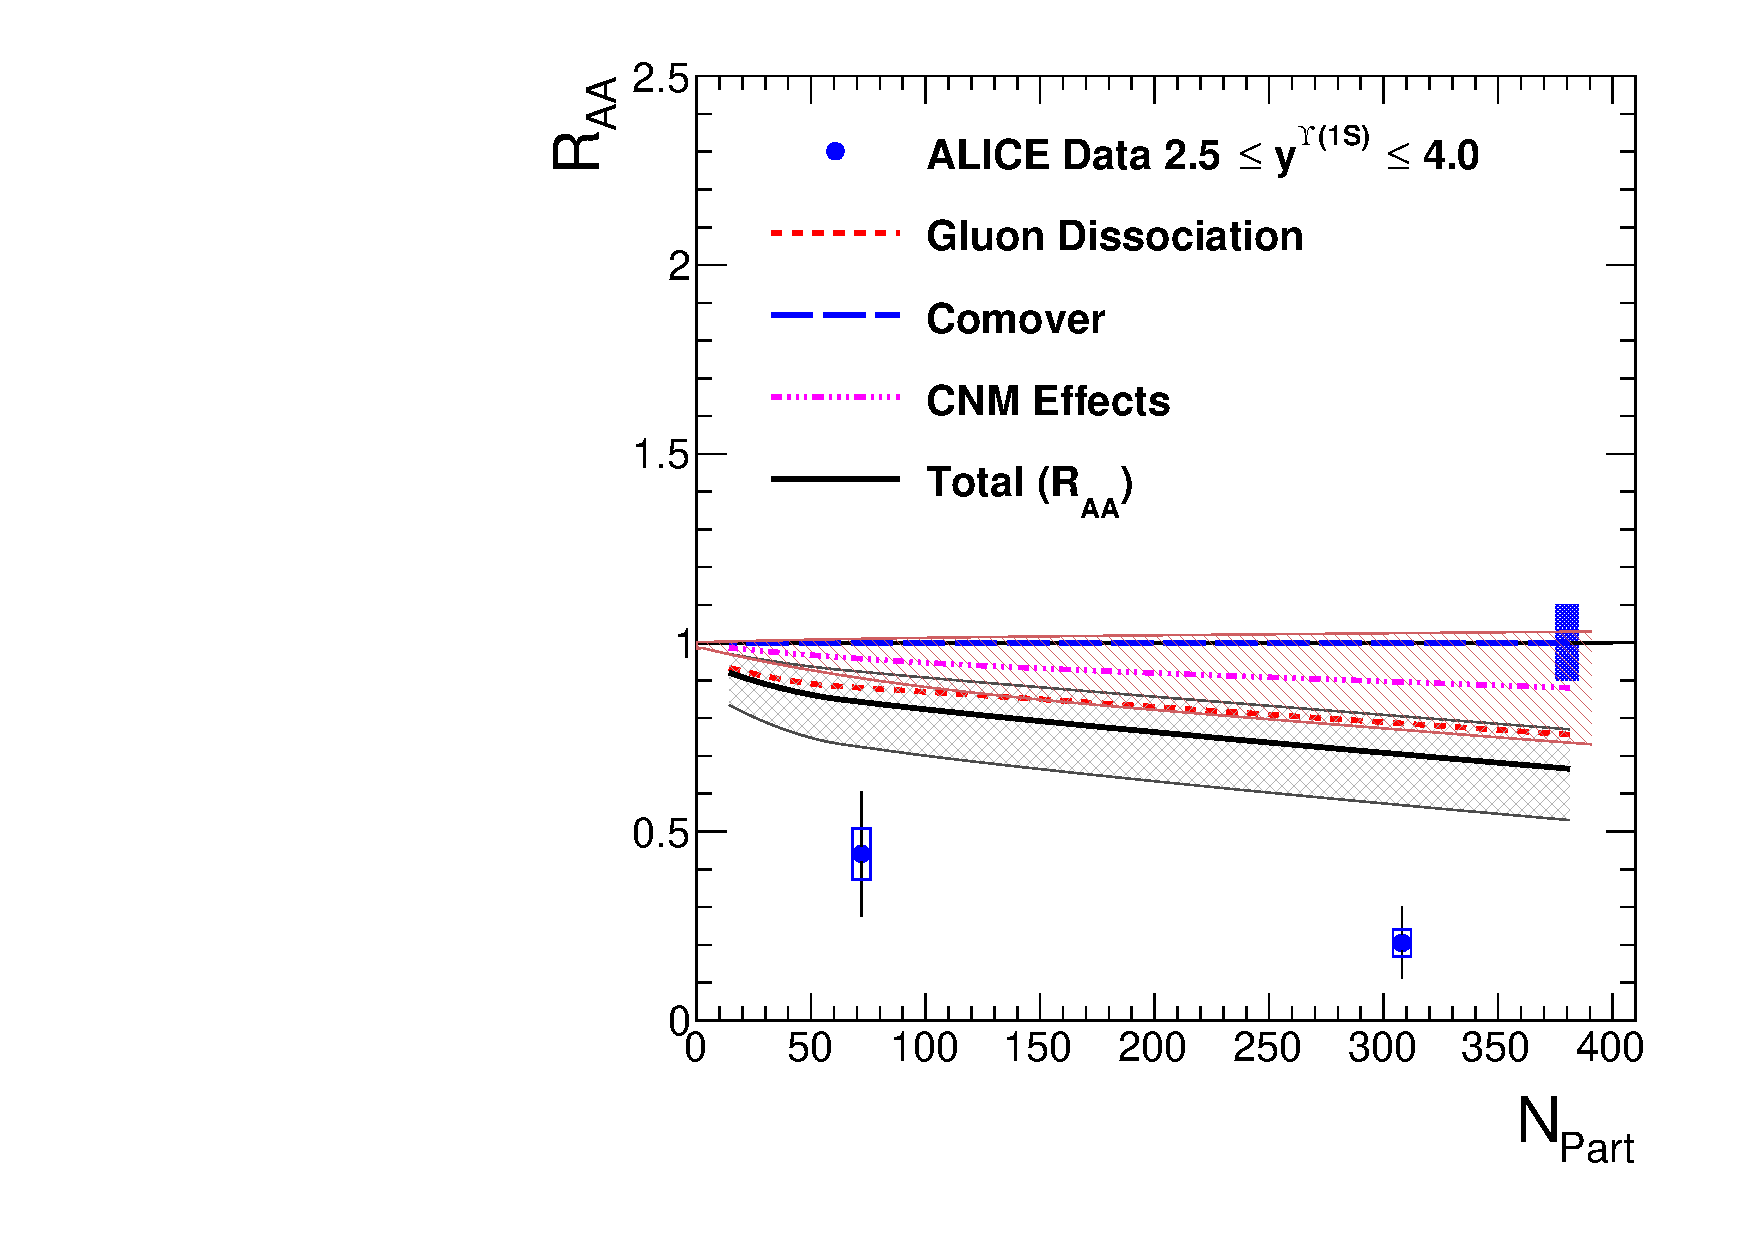
\includegraphics[width=0.49\textwidth]{Figures/Quarkonia_276TeV/Fig9_ALICE_Y1SRAANPart.pdf}
    \caption{(Color online) Calculated nuclear modification factor ($R_{AA}$) compared with 
      ALICE $\Upsilon$(1S) measurement in forward rapidity.}
    \label{fig:ALICERaaY}
  \end{figure}




Figure~\ref{fig:UpsilonRaa} (a) demonstrates the contributions from different processes to the 
centrality dependence of the $\Upsilon$(1S) nuclear modification factor, along with the midrapidity 
data from CMS~\cite{Chatrchyan:2012lxa}. The calculations underestimate the suppression but reproduce 
the shape of centrality dependence. This may be due to the feed down effects from the excited states. 
Figure~\ref{fig:UpsilonRaa} (b) shows the same for the $\Upsilon$(2S) nuclear modification factor
along with the CMS measurements at midrapidity. The excited $\Upsilon$(2S) states 
are highly suppressed. The effect of regeneration, not shown, is negligible 
for the $\Upsilon$ states. 
{\color{black} Figure~\ref{fig:ALICERaaY} shows the forward rapidity 
  ALICE measurement of the $\Upsilon$(1S) nuclear modification factor \cite{Abelev:2014nua}
  along with our calculations. The suppression due to thermal gluon dissociation is smaller 
  than the measured suppression which may be due to the effect of feed down from the $\Upsilon$(2S)
  and higher states.} 
{\color{black} However the measurement is consistent with the suppression of $\Upsilon$(2S) and  
  $\Upsilon$(3S) contribution, along with suppression of the $\Upsilon$(1S) by gluon 
  dissociation.
}


%%%%%%%%%%%%%%%%%%%%%%%%%%%%%%%%%%%%%%%%%%%%%%%%%%%%%%%% 5.02 TeV %%%%%%%%%%%%%%%%%%%%%%%%%%%%%%%%%%%%%%%%%
\begin{figure}
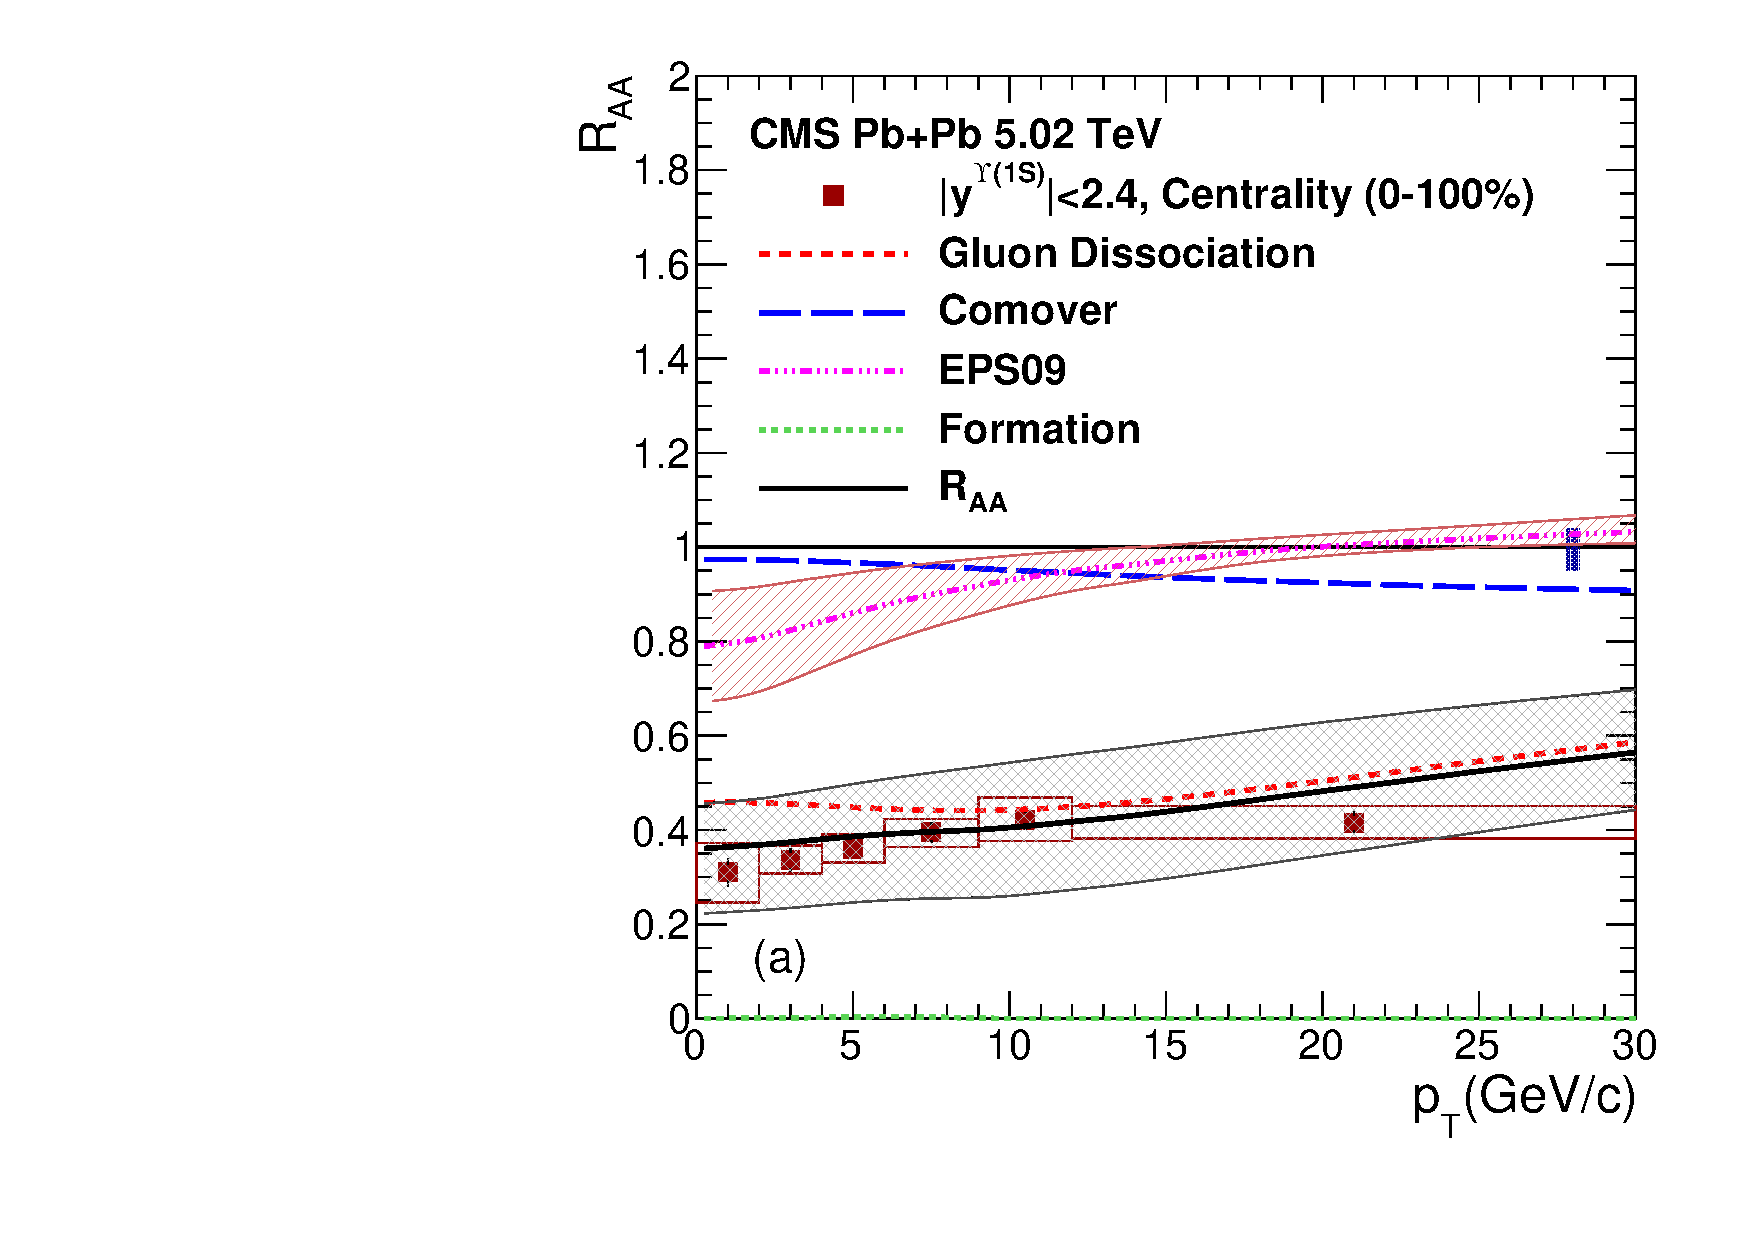
\includegraphics[width=0.49\textwidth]{Figures/Quarkonia_502TeV/Fig7a_Y1S_CMS_RAAPt_Shade.pdf}
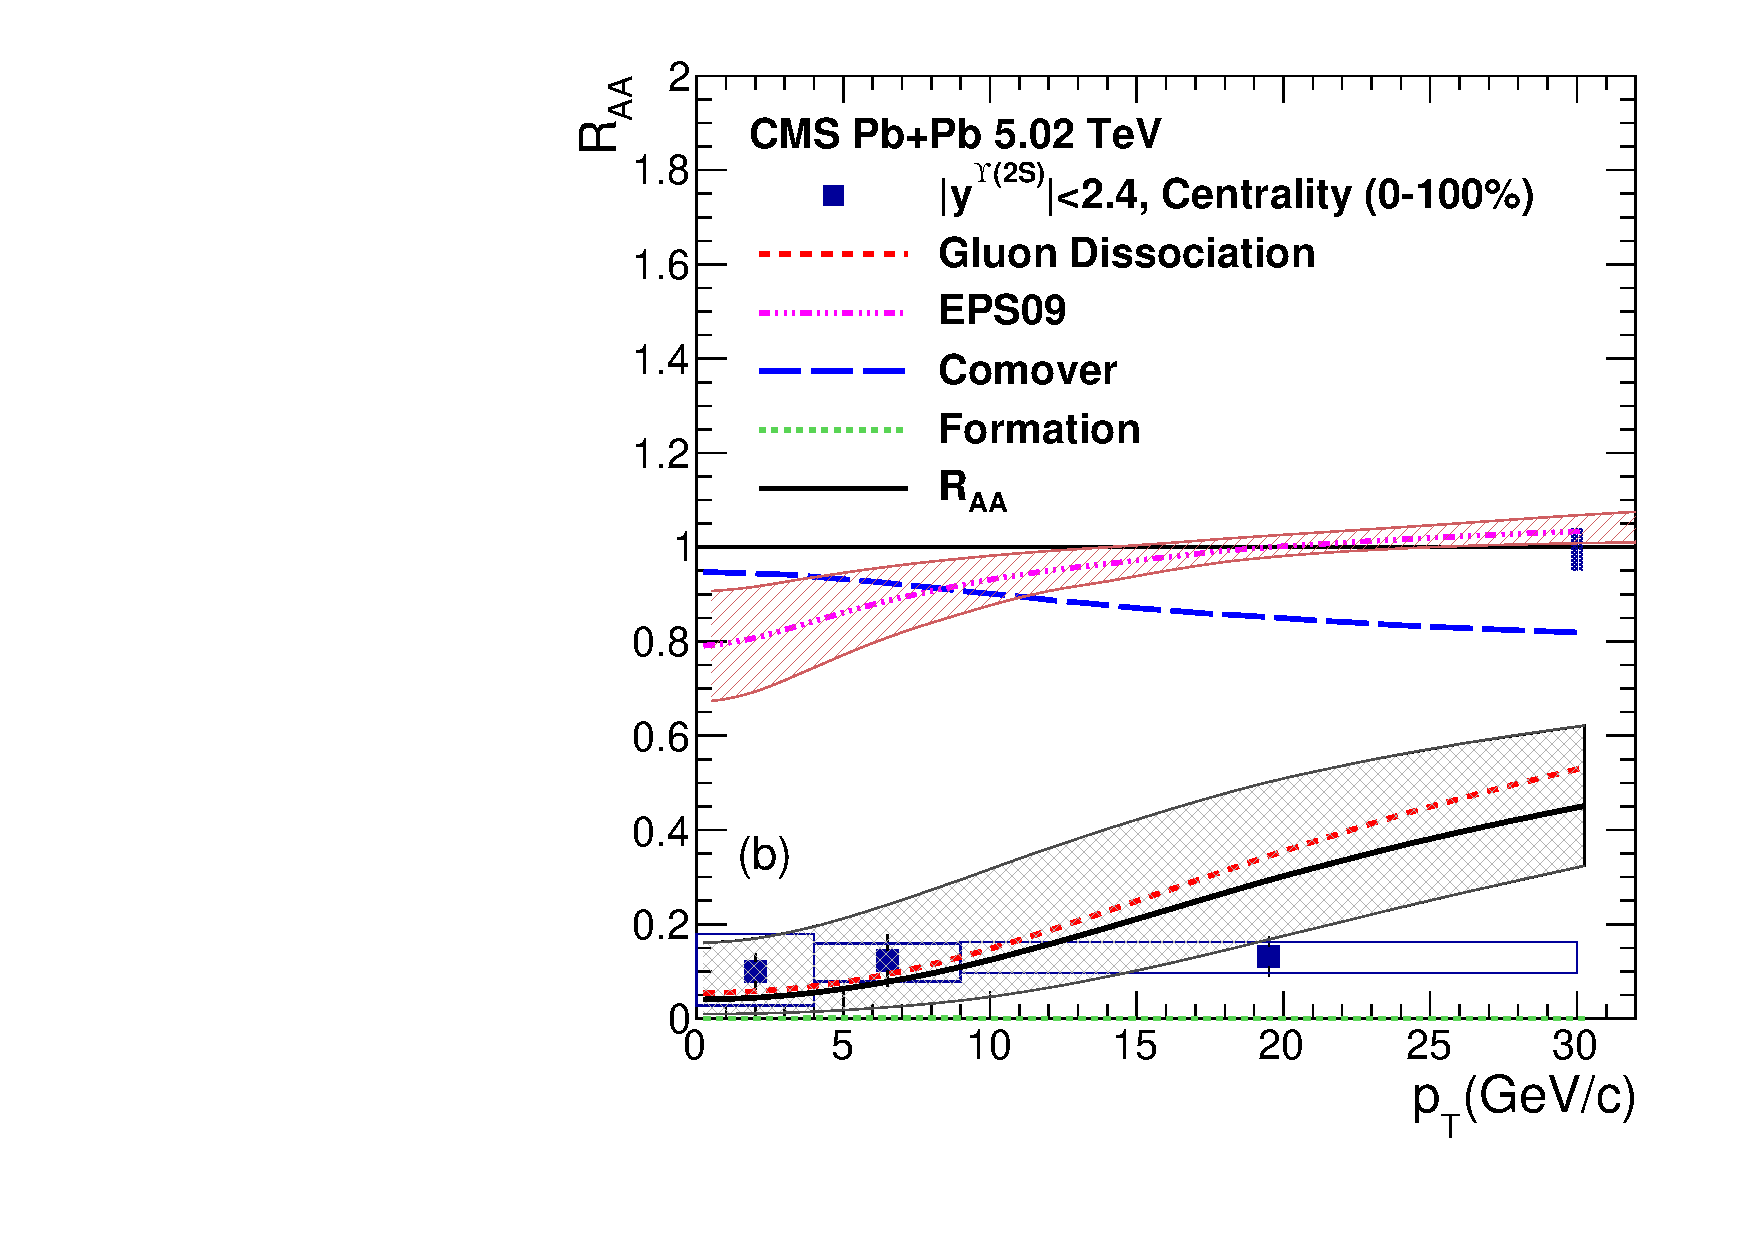
\includegraphics[width=0.49\textwidth]{Figures/Quarkonia_502TeV/Fig7b_Y2S_CMS_RAAPt_Shade.pdf}
\caption{(Color online) Calculated nuclear modification factor ($R_{AA}$) of (a) $\Upsilon$(1S) and 
  (b) $\Upsilon$(2S) as a function of $p_{T}$ 
  compared with CMS measurements~\cite{Sirunyan:2018nsz}.
The global uncertainty in $R_{AA}$ is shown as a band around the line at 1.
}
\label{fig:UpsilonRaaPtCMS}
\end{figure}



\begin{figure}
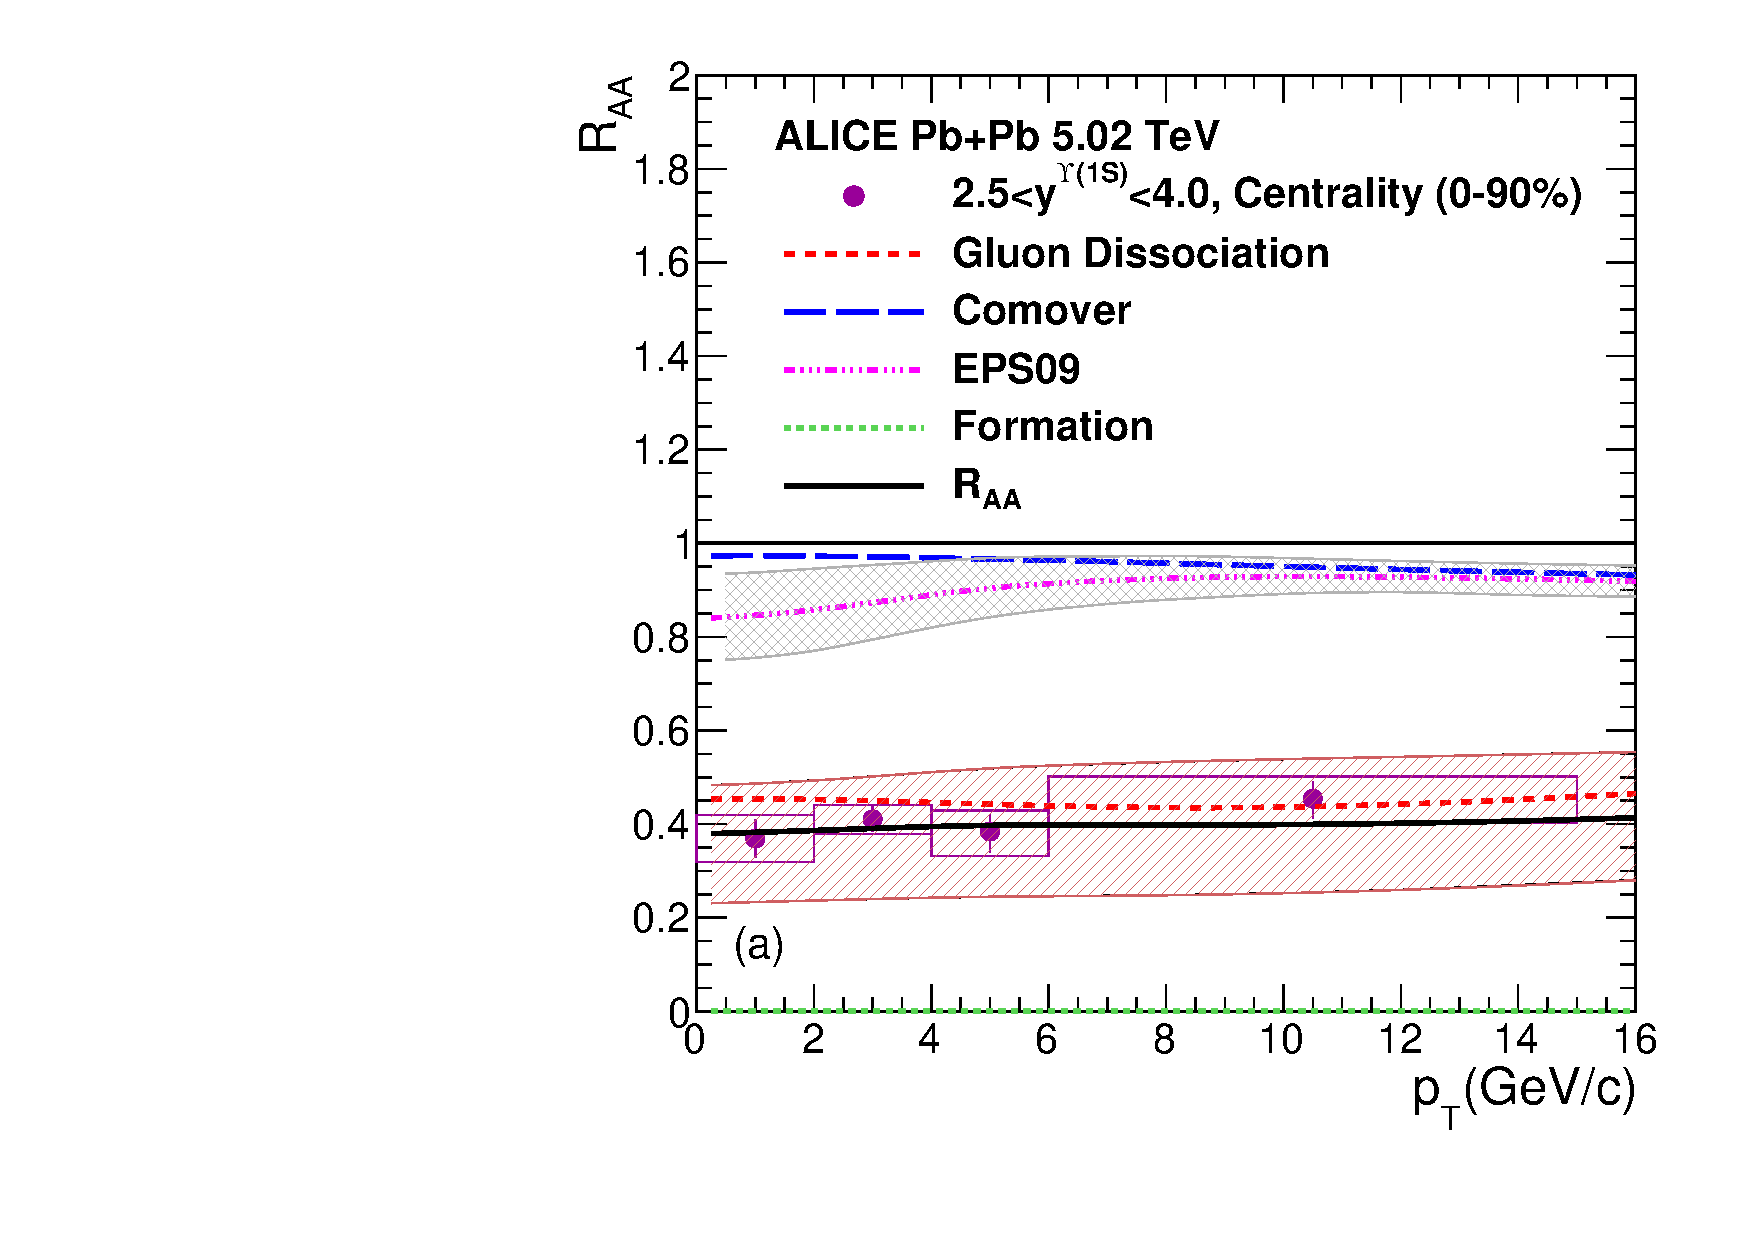
\includegraphics[width=0.49\textwidth]{Figures/Quarkonia_502TeV/Fig8a_ALICE_Y1SRAAPt_Shade.pdf}
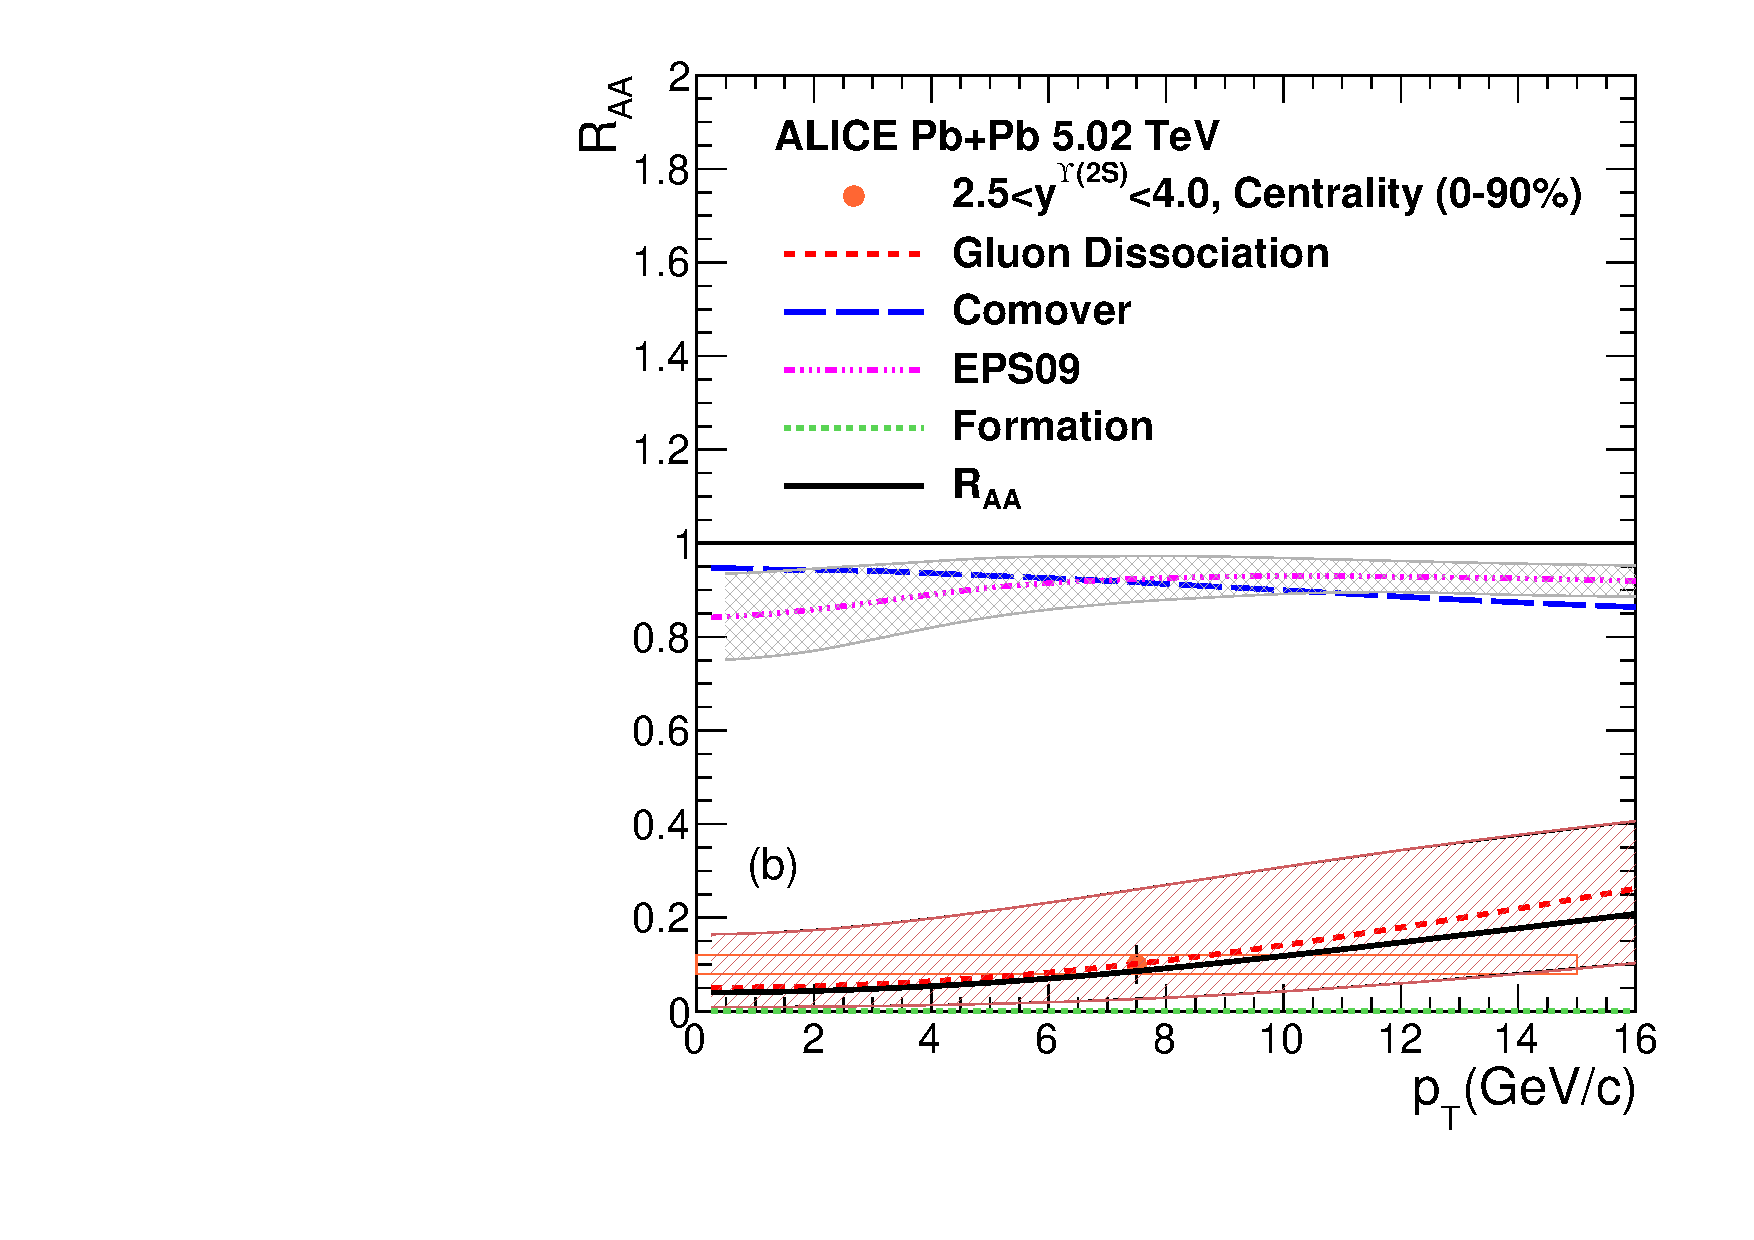
\includegraphics[width=0.49\textwidth]{Figures/Quarkonia_502TeV/Fig8b_ALICE_Y2SRAAPt_Shade.pdf}
\caption{(Color online) Calculated nuclear modification factor ($R_{AA}$) of (a) $\Upsilon$(1S) and 
  (b) $\Upsilon$(2S) as a function of $p_{T}$ in the kinematic range of ALICE detector at LHC ~\cite{ALICE:Y5TeV}.
  The global uncertainty in $R_{AA}$ is shown as a band around the line at 1.
} 
\label{fig:UpsilonRaaPtALICE}
\end{figure}

\begin{figure}
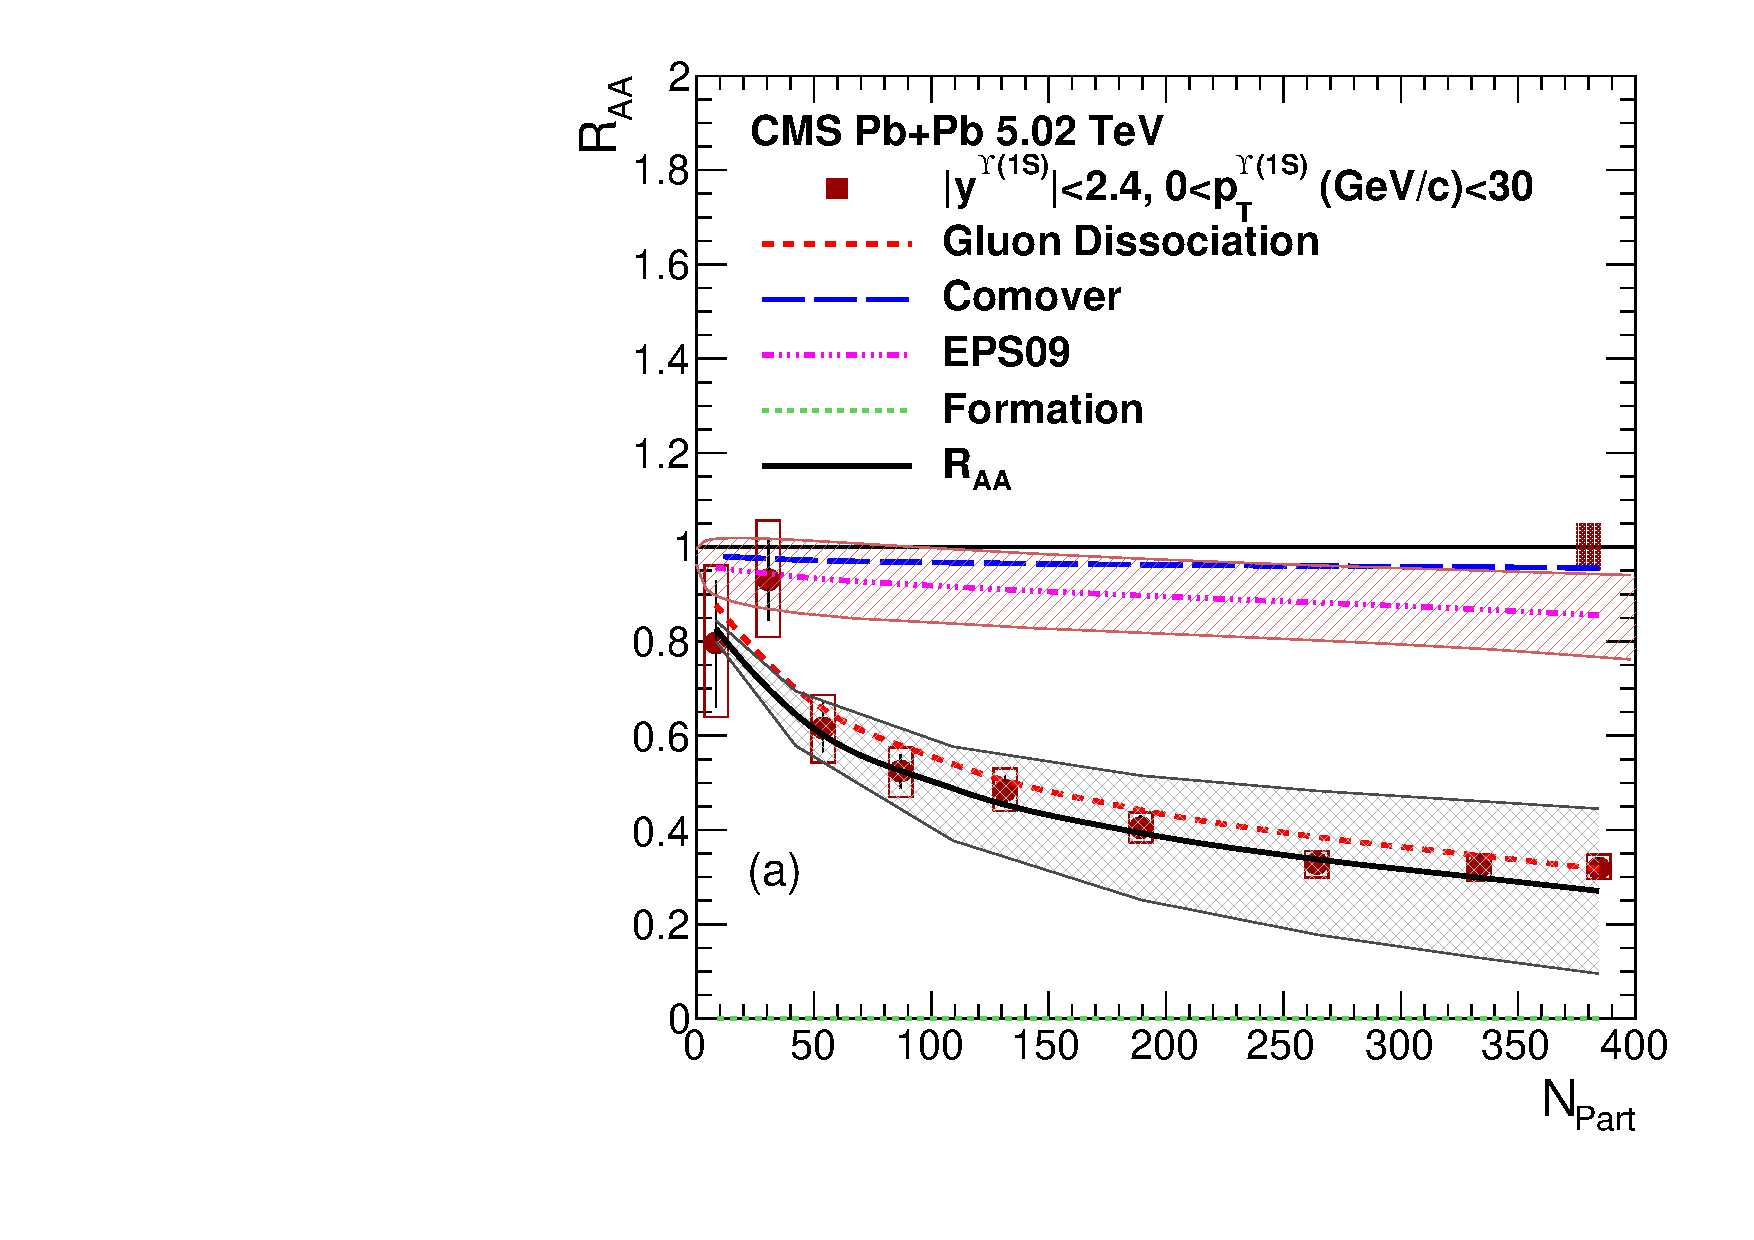
\includegraphics[width=0.49\textwidth]{Figures/Quarkonia_502TeV/Fig9a_CMS_Y1SRAANPart_Shade.pdf}
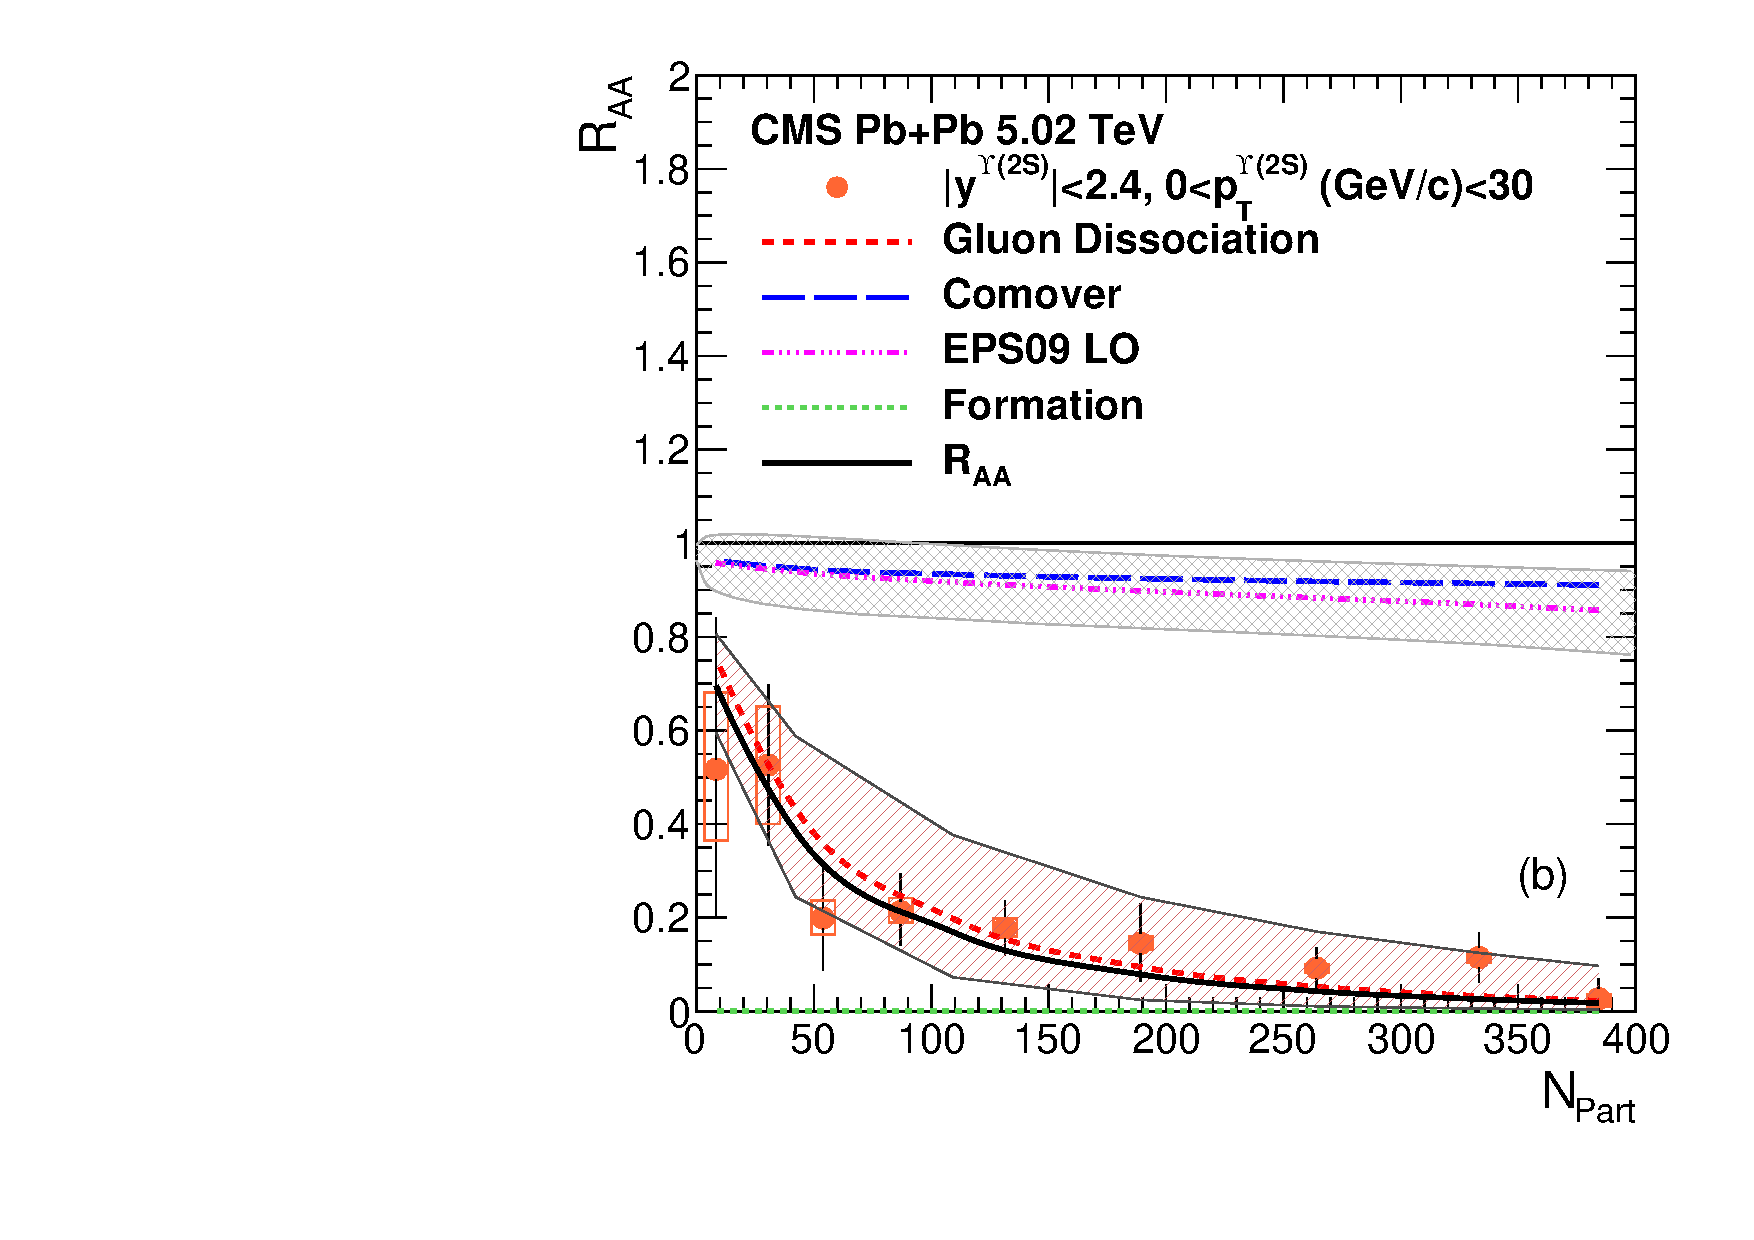
\includegraphics[width=0.49\textwidth]{Figures/Quarkonia_502TeV/Fig9b_CMS_Y2SRAANPart_Shade.pdf}
\caption{(Color online) Calculated nuclear modification factor ($R_{AA}$) of 
  (a) $\Upsilon$(1S) and (b) $\Upsilon$(2S) as a function of centrality of the 
  collisions compared with the CMS measurements~\cite{Sirunyan:2018nsz}.%\cite{CMS:2017ucd}.
  The global uncertainty in $R_{AA}$ is shown as a band around the line at 1.
}
\label{fig:UpsilonRaaNPartCMS}
\end{figure}


Figure~\ref{fig:UpsilonRaaPtCMS}(a) and (b) show the calculations of contributions to
the nuclear modification factor, $R_{AA}$, for the $\Upsilon$(1S) and $\Upsilon$(2S)
respectively as a function of $p_T$ compared with the mid rapidity measurements from
CMS~\cite{Sirunyan:2018nsz}.  
The gluon dissociation mechanism combined with the pion dissociation and shadowing
corrections gives good description of data in mid $p_{T}$ range ($p_{T}\approx$ 5-10 GeV/c)
for both $\Upsilon$(1S) and $\Upsilon$(2S).
The contribution from the regenerated $\Upsilon$s is negligible even at LHC energies.
Our calculations under-predict the suppression observed at the highest measured
$p_{T}$ for $\Upsilon$(1S) and $\Upsilon$(2S) which is similar for the case
of J/$\psi$.
%The feed-down corrections are applied in our calculations following the similar
%procedure as in Refs.~\cite{Abdulsalam:2012bw,Krouppa:2017jlg}. 
%%%%%%%%% insert the feed-down details here
The states $\Upsilon$(1S) and $\Upsilon$(2S) also have
feed-down contributions from decays of higher b$\bar{\rm b}$ bound states.
The nuclear modification factor, $R_{AA}$ is obtained taking into account the feed-down corrections as follows
  \begin{equation}
    R_{AA}^{\Upsilon(3S)} = R_{AA}^{\Upsilon(3S)}\\ %\nonumber
  \end{equation}
  \begin{equation}
    R_{AA}^{\Upsilon(2S)} = f_1 R_{AA}^{\Upsilon(2S)} +  f_2 R_{AA}^{\Upsilon(3S)} \\ %\nonumber
  \end{equation}
   \begin{equation}
    R_{AA}^{\Upsilon(1S)} = g_1 R_{AA}^{\Upsilon(1S)} +  g_2 R_{AA}^{\chi_b(1P)} + g_3 R_{AA}^{\Upsilon(2S)} + g_4 R_{AA}^{\Upsilon(3S)}\\ %\nonumber
  \end{equation}
The factors $f$'s and $g$'s are obtained from CDF measurement~\cite{Affolder:1999wm}.
The values of $g_1$, $g_2$, $g_3$ and $g_4$ are 0.509, 0.27, 0.107
and 0.113 respectively. Here $g_4$ is assumed to be the combined fraction of 
$\Upsilon$(3S) and $\chi_b$(2P).
The values of $f_1$ and $f_2$ are taken as 0.50~\cite{Strickland:2011aa}.


Figure~\ref{fig:UpsilonRaaPtALICE}(a) and (b) show the model 
prediction of the nuclear modification factor, $R_{AA}$, for the $\Upsilon$(1S)
and $\Upsilon$(2S) respectively as a function of $p_T$ in the kinematic range
covered by ALICE detector. The ALICE data~\cite{ALICE:Y5TeV} is well described by our model.

Figure~\ref{fig:UpsilonRaaNPartCMS}(a) depicts the calculated 
centrality dependence of the $\Upsilon$(1S) nuclear
modification factor, along with the midrapidity data from CMS~\cite{Sirunyan:2018nsz}.
Our calculations combined with the pion dissociation and shadowing corrections 
gives very good description of the measured data. Figure~\ref{fig:UpsilonRaaNPartCMS}(b)
shows the same for the $\Upsilon$(2S) along with the midrapidity
CMS measurements. The suppression of the excited $\Upsilon$(2S) states 
is also well described by our model. As stated earlier, the effect of regeneration is
negligible for $\Upsilon$ states. 

Figure~\ref{fig:UpsilonRaaNPartALICE}(a) shows the forward rapidity ALICE
measurement of the $\Upsilon$(1S) nuclear modification factor~\cite{ALICE:Y5TeV}
along with our calculations. The suppression due to thermal gluon dissociation 
describes the measured data after including the comover and shadowing corrections.
Figure~\ref{fig:UpsilonRaaNPartALICE}(b) shows the calculations for the
$\Upsilon$(2S) nuclear modification factor in ALICE detector kinematic range.
The suppression due to thermal gluon dissociation describes the
ALICE measurements after including the comover and shadowing corrections.


  %%%%%%%%%%%%%%%%%%%%%%%%%%%%%%%%%%%%%%%%%%%%%%%%%%%%%%%%%%%%%%%%%%%%%%%%%%%%%%%%%%%%%%%%
\subsubsection{Statistical (re) generation models}
{\color{red} We can include the regenration part from our calculations. These effects are also small.}


%\subsubsection{Non-equilibrium effects on quarkonium suppression}
%\subsubsection{Collisional dissociation of quarkonia from final-state interactions}

\subsubsection{Comover models}

%\section{hadronic comovers}
  The suppression of quarkonia by comoving pions can be calculated by folding the quarkonium-pion
dissociation cross section $\sigma_{\pi Q}$ over thermal pion distributions \cite{Vogt:1988fj}. 
It is expected  that at LHC energies, the comover cross section will be small~\cite{Lourenco:2008sk}.
{\color{black}
The pion-quarkonia cross section is calculated by convoluting the gluon-quarkonia cross section $\sigma_D$
over the gluon distribution inside the pion~\cite{Arleo:2001mp},
\begin{equation}
\sigma_{\pi Q} (p_{\pi}) = {p_+^2 \over 2(p_\pi^2 - m_\pi^2)} \int_0^1 \, dx \, G(x) \, \sigma_D(xp_+/\sqrt {2}),
\end{equation}
where $p_+ = (p_\pi + \sqrt{p_\pi^2-m_\pi^2})/\sqrt{2}$. The gluon distribution, $G(x)$, inside a pion is 
given by the GRV parameterization~\cite{Gluck:1991ey}. 
The pion momentum $p_\pi$ is related to center of mass energy $\sqrt{s}$ of pion-$J/\psi$ system by 
$p_\pi = (s-M_Q^2-m_\pi^2)/(2M_Q)$.}
The dissociation rate $\lambda_{D_{\pi}}$  can be written as
\begin{eqnarray}
  \lambda_{D_{\pi}} \, \rho_{\pi} & = & \frac{g_\pi}{(2\pi)^{3}} \int d^{3}p_{\pi} f_{\pi}(p) \sigma_{\pi Q} (s) v_{\rm rel} (s) \\ \nonumber
                              & = &\frac{g_\pi}{(2\pi)^{3}} \int\,dp_{\pi}\,2\pi p_{\pi}^{2} f_{\pi}(p_{\pi}) \int\,d{\rm cos}\theta\,\sigma_{\pi Q}(s) \, v_{\rm rel}(s) \Theta(s-4m_{D}^{2}),  \\\nonumber
\end{eqnarray}
where $f_{\pi}(p_{\pi},T)$ is the thermal pion distribution. The  pion density $\rho_{\pi}$ is 
\begin{eqnarray}
\rho_\pi =\frac{g_\pi}{(2\pi)^{3}} \int d^3p_{\pi} \, f_{\pi}(p_{\pi}). 
\end{eqnarray}
The survival probability from pion collisions at freeze-out time $\tau_f$ is written as
\begin{equation}
S_\pi(p_T) = \exp \left( {-\int_{\tau_0}^{\tau_f} \,d\tau\,(1-f(\tau)) \lambda_{D_{\pi}}(T,p_T)\,\rho_{\pi}(T)} \right).
\end{equation}
The hadronic fraction (1-$f(\tau)$) is zero in QGP phase.
The probability $S_\pi(p_T)$ multiplies $S(p_T)$ in Eq.~(\ref{raa}).



\subsubsection{Summary of theoretical models for experimental comparison}

{\color{red} We will write the summary for all different type of quarkonia model here.}

